\documentclass[hide notes,intlimits,usenames,dvipsnames]{beamer}

\mode<presentation>
{
  \usetheme{Singapore}
  \usefonttheme{professionalfonts}
  \setbeamertemplate{blocks}[rounded][shadow=true]
  \setbeamercovered{transparent}
  \setbeamertemplate{footline}[frame number]
}

% load packages
\usepackage[english]{babel}
\usepackage[latin1]{inputenc}
\usepackage[T1]{fontenc}
\usepackage{lmodern}
\usepackage[multidot]{grffile}
\usepackage{amsmath,verbatim,empheq,xspace}

\usepackage{tikz}
\usetikzlibrary{shapes,shadows,fadings}
\usetikzlibrary{decorations.markings,decorations.pathreplacing}
\usetikzlibrary{arrows,arrows.meta}

%\usepackage{animate}

\usepackage[noend]{algpseudocode}
\usepackage{listings}

% see http://tex.stackexchange.com/questions/86188/labelling-with-arrows-in-an-automated-way

\newif\ifclipme\clipmetrue
\tikzset{labelstyle/.style={LabelStyle/.append style={#1}},linestyle/.style={LineStyle/.append style={#1}}}
\tikzset{LabelStyle/.initial={},LineStyle/.initial={}}

\newcommand{\mathWithDescription}[4][]{{%
    \tikzset{#1}%
    \tikz[baseline]{
        \node[draw=red,rounded corners,anchor=base] (m#4) {$\displaystyle#2$};
        \ifclipme\begin{pgfinterruptboundingbox}\fi
            \node[above of=m#4,font=\strut, LabelStyle] (l#4) {#3};
            \draw[-,red, LineStyle] (l#4) to (m#4);
        \ifclipme\end{pgfinterruptboundingbox}\fi
    }%
}}

\newcommand{\mathWithDescriptionStarred}[3][]{{%
    \clipmefalse%
    \mathWithDescription[#1]{#2}{#3}{\themathLabelNode}%
}}

\newcounter{mathLabelNode}

\newcommand{\mathLabelBox}[3][]{%
   \stepcounter{mathLabelNode}%
   \mathWithDescription[#1]{#2}{#3}{\themathLabelNode}%
   \vphantom{\mathWithDescriptionStarred[#1]{#2}{#3}{\themathLabelNode}}%
}

\definecolor{dark red}{HTML}{E41A1C}
\definecolor{dark green}{HTML}{4DAF4A}
\definecolor{dark violet}{HTML}{984EA3}
\definecolor{dark blue}{HTML}{084594}
\definecolor{dark orange}{HTML}{FF7F00}
\definecolor{light blue}{HTML}{377EB8}
\definecolor{light red}{HTML}{FB9A99}
\definecolor{light violet}{HTML}{CAB2D6}

\newcommand{\CC}{\mathbb{C}}
\newcommand{\NN}{\mathbb{N}}
\newcommand{\RR}{\mathbb{R}}
\newcommand{\ZZ}{\mathbb{Z}}

\newcommand{\Kcal}{\mathcal{K}}
\newcommand{\Xcal}{\mathcal{X}}

\newcommand{\bF}{\mathbf{F}}
\newcommand{\bQ}{\mathbf{Q}}
\newcommand{\bU}{\mathbf{U}}
\newcommand{\bX}{\mathbf{X}}

\newcommand{\bb}{\mathbf{b}}
\newcommand{\be}{\mathbf{e}}
\newcommand{\bq}{\mathbf{q}}
\newcommand{\br}{\mathbf{r}}
\newcommand{\bs}{\mathbf{s}}
\newcommand{\bu}{\mathbf{u}}
\newcommand{\bv}{\mathbf{v}}
\newcommand{\bw}{\mathbf{w}}
\newcommand{\bx}{\mathbf{x}}
\newcommand{\by}{\mathbf{y}}
\newcommand{\bz}{\mathbf{z}}

\newcommand{\Div}{\nabla\cdot}
\newcommand{\eps}{\epsilon}
\newcommand{\grad}{\nabla}
\newcommand{\lap}{\triangle}
\renewcommand{\bar}{\overline}

\newcommand{\ip}[2]{\ensuremath{\left<#1,#2\right>}}


\newcommand{\FM}{F$\begin{smallmatrix} \text{D} \\ \text{E} \end{smallmatrix}$M\xspace}


\newenvironment{transbox}[1][]{%
\begin{tikzpicture}
\node[drop shadow,rounded corners,text width=\textwidth,fill=white, fill opacity=#1,text opacity=1] \bgroup
}{
\egroup;\end{tikzpicture}}


\title{Optimal solvers for partial differential equations}

\author[Bueler]{Ed Bueler}

\institute[UAF]{
  \scriptsize Dept of Mathematics and Statistics and Geophysical Institute \\

  University of Alaska Fairbanks
}

%\titlegraphic{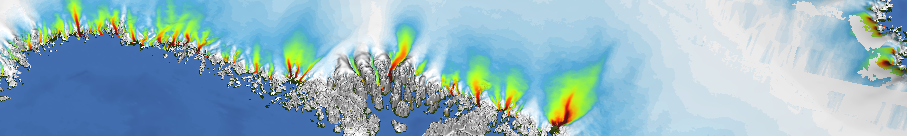
\includegraphics[width=\textwidth]{andycoast.png}}

\beamertemplatenavigationsymbolsempty   % remove faint and silly navigation symbols at bottom
\renewcommand{\insertnavigation}[1]{}   % remove section headings from top of each slide

\setbeamerfont{date}{size=\scriptsize}
\date{}

\AtBeginSection[]
{
  \begin{frame}<beamer>
    \frametitle{Outline}
    %\tableofcontents[currentsection,hideallsubsections]
    \tableofcontents[currentsection]
  \end{frame}
}


\begin{document}

%\graphicspath{{../../old/commonfigs/}}

\begin{frame}
    \vspace{10mm}
    \titlepage
    \begin{center}
    \tiny DMS Colloquium \quad 28 November, 2017
    \end{center}
\end{frame}

%\begin{frame}
%    \frametitle{Outline}
%    \tableofcontents
%\end{frame}

\begin{frame}{why this talk?}

\begin{itemize}
\item I have been thinking about what is the \emph{goal} when numerically solving differential equations
\item there are reliable black boxes for ODE IVPs
	\begin{itemize}
	\item[$\circ$] \texttt{ode45} in \textsc{Matlab}
	\end{itemize}
\item how would you build a good PDE black box?
\end{itemize}
\end{frame}


\section{how to approximately solve a PDE}

\begin{frame}{Poisson equation}

\begin{itemize}
\item for much of this talk I'll use two example PDE problems

\bigskip
\item[\textbf{1.}] \emph{Poisson equation} with Dirichlet boundary conditions:
	    $$- \grad^2 u = f \qquad \text{ on } \Omega \subset \RR^d \text{ with } u\big|_{\partial \Omega} = g,$$
    \vspace{-5mm}
	\begin{itemize}
	\item[$\circ$] a linear elliptic PDE problem in dimension $d=2$ or $d=3$
	\item[$\circ$] recall that $\grad^2 u = \Div \left(\grad u\right) = u_{xx}+u_{yy}+u_{zz}$
	\item[$\circ$] source $f(x,y,z)$ given
	\item[$\circ$] boundary values $g(x,y,z)$ given
	\item[$\circ$] will use various domains $\Omega$ including a square, a cube, and
		\begin{itemize}
        \item a snowflake fractal \hspace{0.3in} \begin{tikzpicture}[scale=0.8,baseline] \begin{tikzpicture}[scale=1.0,baseline]
  \draw[line width=1.000000pt] (-0.866025,0.500000) -- (-0.673575,0.500000);
  \draw[line width=1.000000pt] (-0.673575,0.500000) -- (-0.577350,0.666667);
  \draw[line width=1.000000pt] (-0.577350,0.666667) -- (-0.481125,0.500000);
  \draw[line width=1.000000pt] (-0.481125,0.500000) -- (-0.288675,0.500000);
  \draw[line width=1.000000pt] (-0.288675,0.500000) -- (-0.192450,0.666667);
  \draw[line width=1.000000pt] (-0.192450,0.666667) -- (-0.288675,0.833333);
  \draw[line width=1.000000pt] (-0.288675,0.833333) -- (-0.096225,0.833333);
  \draw[line width=1.000000pt] (-0.096225,0.833333) -- (0.000000,1.000000);
  \draw[line width=1.000000pt] (0.000000,1.000000) -- (0.096225,0.833333);
  \draw[line width=1.000000pt] (0.096225,0.833333) -- (0.288675,0.833333);
  \draw[line width=1.000000pt] (0.288675,0.833333) -- (0.192450,0.666667);
  \draw[line width=1.000000pt] (0.192450,0.666667) -- (0.288675,0.500000);
  \draw[line width=1.000000pt] (0.288675,0.500000) -- (0.481125,0.500000);
  \draw[line width=1.000000pt] (0.481125,0.500000) -- (0.577350,0.666667);
  \draw[line width=1.000000pt] (0.577350,0.666667) -- (0.673575,0.500000);
  \draw[line width=1.000000pt] (0.673575,0.500000) -- (0.866025,0.500000);
  \draw[line width=1.000000pt] (0.866025,0.500000) -- (0.769800,0.333333);
  \draw[line width=1.000000pt] (0.769800,0.333333) -- (0.866025,0.166667);
  \draw[line width=1.000000pt] (0.866025,0.166667) -- (0.673575,0.166667);
  \draw[line width=1.000000pt] (0.673575,0.166667) -- (0.577350,0.000000);
  \draw[line width=1.000000pt] (0.577350,0.000000) -- (0.673575,-0.166667);
  \draw[line width=1.000000pt] (0.673575,-0.166667) -- (0.866025,-0.166667);
  \draw[line width=1.000000pt] (0.866025,-0.166667) -- (0.769800,-0.333333);
  \draw[line width=1.000000pt] (0.769800,-0.333333) -- (0.866025,-0.500000);
  \draw[line width=1.000000pt] (0.866025,-0.500000) -- (0.673575,-0.500000);
  \draw[line width=1.000000pt] (0.673575,-0.500000) -- (0.577350,-0.666667);
  \draw[line width=1.000000pt] (0.577350,-0.666667) -- (0.481125,-0.500000);
  \draw[line width=1.000000pt] (0.481125,-0.500000) -- (0.288675,-0.500000);
  \draw[line width=1.000000pt] (0.288675,-0.500000) -- (0.192450,-0.666667);
  \draw[line width=1.000000pt] (0.192450,-0.666667) -- (0.288675,-0.833333);
  \draw[line width=1.000000pt] (0.288675,-0.833333) -- (0.096225,-0.833333);
  \draw[line width=1.000000pt] (0.096225,-0.833333) -- (0.000000,-1.000000);
  \draw[line width=1.000000pt] (0.000000,-1.000000) -- (-0.096225,-0.833333);
  \draw[line width=1.000000pt] (-0.096225,-0.833333) -- (-0.288675,-0.833333);
  \draw[line width=1.000000pt] (-0.288675,-0.833333) -- (-0.192450,-0.666667);
  \draw[line width=1.000000pt] (-0.192450,-0.666667) -- (-0.288675,-0.500000);
  \draw[line width=1.000000pt] (-0.288675,-0.500000) -- (-0.481125,-0.500000);
  \draw[line width=1.000000pt] (-0.481125,-0.500000) -- (-0.577350,-0.666667);
  \draw[line width=1.000000pt] (-0.577350,-0.666667) -- (-0.673575,-0.500000);
  \draw[line width=1.000000pt] (-0.673575,-0.500000) -- (-0.866025,-0.500000);
  \draw[line width=1.000000pt] (-0.866025,-0.500000) -- (-0.769800,-0.333333);
  \draw[line width=1.000000pt] (-0.769800,-0.333333) -- (-0.866025,-0.166667);
  \draw[line width=1.000000pt] (-0.866025,-0.166667) -- (-0.673575,-0.166667);
  \draw[line width=1.000000pt] (-0.673575,-0.166667) -- (-0.577350,0.000000);
  \draw[line width=1.000000pt] (-0.577350,0.000000) -- (-0.673575,0.166667);
  \draw[line width=1.000000pt] (-0.673575,0.166667) -- (-0.866025,0.166667);
  \draw[line width=1.000000pt] (-0.866025,0.166667) -- (-0.769800,0.333333);
  \draw[line width=1.000000pt] (-0.769800,0.333333) -- (-0.866025,0.500000);
\end{tikzpicture}
 \end{tikzpicture}
        \end{itemize}
	\item[$\circ$] the solution $u(x,y,z)$ of $- \grad^2 u = 1$ with $g=0$ gives the expected time for a Brownian motion to first hit $\partial\Omega$
	\end{itemize}
\end{itemize}
\end{frame}


\begin{frame}{minimal surface equation}

\begin{itemize}
\item[\textbf{2.}] \emph{minimal surface equation (MSE)} with Dirichlet b.c.s:
	    $$- \grad\cdot \left(\frac{\grad u}{\sqrt{1 + |\grad u|^2}}\right) = 0  \qquad \text{ with } u\big|_{\partial \Omega} = g.$$
    \vspace{-2mm}
	\begin{itemize}
	\item[$\circ$] a nonlinear elliptic PDE in 2D
	\item[$\circ$] here: square domain $\Omega = [0,1] \times [0,1]$
	\item[$\circ$] the solution $u(x,y)$ gives the height of a zero-gravity soap bubble which spans a wire frame with height $z=g(x,y)$:
	\end{itemize}

\begin{center}
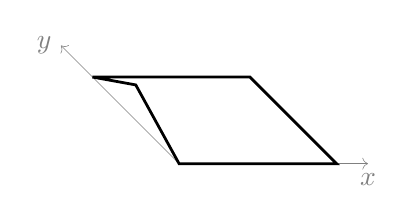
\begin{tikzpicture}[scale=2.0]
  \draw[->,gray,very thin] (0.0,0.0) -- (1.2,0.0) node[below] {$x$};
  \draw[->,gray,very thin] (0.0,0.0) -- (-0.75,0.75) node[left] {$y$};
  \draw[line width=1.0pt] (0.0,0.0) -- (1.0,0.0) -- (0.45,0.55) -- (-0.55,0.55) -- (-0.275,0.5) -- cycle;
\end{tikzpicture}
\end{center}
\end{itemize}
\end{frame}


\begin{frame}{today's talk: mostly elliptic PDEs}

both examples {\color{Blue} \textbf{1}} \& {\color{Blue} \textbf{2}}
\begin{itemize}
\item are well-posed elliptic PDE BVPs
\item seek solution $u$ from an \alert{$\infty$-dimensional vector space}
\item \emph{main idea}: a PDE BVP is a system of $\infty$ eqns in $\infty$ unknowns
\end{itemize}

\bigskip\bigskip\bigskip

\scriptsize
fine print:
\begin{itemize}
\item both examples derivable from variational principles, thus well-posed
\item the ``$\infty$-dimensional vector space'' is a Sobolev space such as $H^1(\Omega)$
%\item \emph{numerically}, nonlinear elliptic PDE BVPs are representative of the hardest class of PDE problems because they arise as the time-step problems in the (harder) stiff time-dependent case
%\item \dots but smoothness of the solution matters \emph{a lot} to numerical difficulty
\end{itemize}
\end{frame}


\begin{frame}{approximation: finite difference method}
\begin{itemize}
\item most problems are not solvable exactly, so we
	\begin{itemize}
	\item[$\circ$] \alert{approximate by $N$ equations in $N$ unknowns}
	\item[$\circ$] where $N\in\ZZ^+$ so $N \ll \infty$

    \smallskip
	\item[$\circ$] of course, some problems can be solved exactly
        \begin{itemize}
        \item[\emph{example}.]  $u(x,y)=x^2-y^2$ solves $\grad^2 u = 0$
        \end{itemize}
	\end{itemize}
\item one method is \emph{finite differences} (FDM), based on
	    $$f'(x) = \lim_{h \to 0} \frac{f(x+h)-f(x)}{h} \approx \frac{f(x+h)-f(x)}{h}$$
\item as used for the 2D Poisson equation:
	    $$u_{xx}+u_{yy} \approx \frac{u_{i+1,j} + u_{i-1,j} + u_{i,j+1} + u_{i,j-1} - 4 u_{ij}}{h^2}$$
\end{itemize}
\end{frame}


\begin{frame}{structured grids}
\begin{itemize}
\item for a much of this talk I'll use \emph{structured grids}
	\begin{itemize}
	\item[$\circ$] i.e.~products of grids in 1D
	\end{itemize}
\item sequence of such grids $\Omega^{(k)}$; the \emph{level} $k$ grid has
	\begin{itemize}
	\item[$\circ$] equal spacing $h_k$ in each direction
    \item[$\circ$] $N_k = O(h_k^{-d})$ grid points in $d$ dimensions
	    \begin{itemize}
	    \item typically: $N_{k+1} = 2^d N_k$
	    \end{itemize}
	\end{itemize}

\bigskip
\begin{tikzpicture}[scale=1.6]
\begin{tikzpicture}[scale=1.6]
  \pgfmathsetmacro\half{1.0/2.0}
  \draw[xstep=\half,ystep=\half,black,thin] (0.0,0.0) grid (1.0,1.0);
  \node at (0.5,-0.25) {$\Omega^{(0)}$};
\end{tikzpicture}
\quad
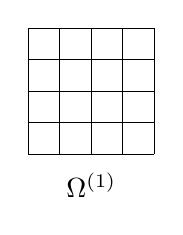
\begin{tikzpicture}[scale=1.6]
  \pgfmathsetmacro\fourth{1.0/4.0}
  \draw[xstep=\fourth,ystep=\fourth,black,thin] (0.0,0.0) grid (1.0,1.0);
  \node at (0.5,-0.25) {$\Omega^{(1)}$};
\end{tikzpicture}
\quad
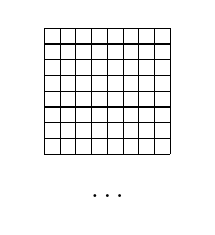
\begin{tikzpicture}[scale=1.6]
  \pgfmathsetmacro\eigth{1.0/8.0}
  \draw[xstep=\eigth,ystep=\eigth,black,thin] (0.0,0.0) grid (1.0,1.0);
  \node at (0.5,-0.25) {$\phantom{\Omega^{(2)}}\dots\phantom{\Omega^{(2)}}$};
\end{tikzpicture}
\quad
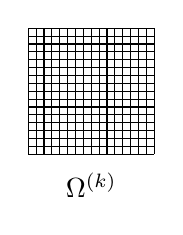
\begin{tikzpicture}[scale=1.6]
  \pgfmathsetmacro\sixteenth{1.0/16.0}
  \draw[xstep=\sixteenth,ystep=\sixteenth,black,thin] (0.0,0.0) grid (1.0,1.0);
  \node at (0.5,-0.25) {$\Omega^{(k)}$};
\end{tikzpicture}

\end{tikzpicture}

\medskip
\item $N_k$ is the number of equations and of unknowns
\item ``increasing resolution'' or ``refinement'' means $h_k \to 0$
\end{itemize}
\end{frame}


\begin{frame}{approximation: finite element method (FEM)}
\begin{itemize}
\item this discretization uses the \emph{weak form} of the PDE
\item example: the weak form for the Poisson equation is
    $$\int_\Omega \grad u \cdot \grad v = \int_\Omega f v \qquad \forall v \in H_0^1(\Omega)$$
    \vspace{-4mm}
	\begin{itemize}
	\item[$\circ$] derivation: multiply PDE by $v$ and integrate by parts
	\end{itemize}
\item FEM is well-suited to unstructured meshes of arbitrary polygonal/polyhedral domains
	\begin{itemize}
	\item[$\circ$] e.g.~triangulate the snowflake:
	\end{itemize}

\begin{center}
\begin{tikzpicture}[scale=1.3,baseline] \begin{tikzpicture}[scale=1.0,baseline]
  \draw[line width=1.000000pt] (-0.866025,0.500000) -- (-0.673575,0.500000);
  \draw[line width=1.000000pt] (-0.673575,0.500000) -- (-0.577350,0.666667);
  \draw[line width=1.000000pt] (-0.577350,0.666667) -- (-0.481125,0.500000);
  \draw[line width=1.000000pt] (-0.481125,0.500000) -- (-0.288675,0.500000);
  \draw[line width=1.000000pt] (-0.288675,0.500000) -- (-0.192450,0.666667);
  \draw[line width=1.000000pt] (-0.192450,0.666667) -- (-0.288675,0.833333);
  \draw[line width=1.000000pt] (-0.288675,0.833333) -- (-0.096225,0.833333);
  \draw[line width=1.000000pt] (-0.096225,0.833333) -- (0.000000,1.000000);
  \draw[line width=1.000000pt] (0.000000,1.000000) -- (0.096225,0.833333);
  \draw[line width=1.000000pt] (0.096225,0.833333) -- (0.288675,0.833333);
  \draw[line width=1.000000pt] (0.288675,0.833333) -- (0.192450,0.666667);
  \draw[line width=1.000000pt] (0.192450,0.666667) -- (0.288675,0.500000);
  \draw[line width=1.000000pt] (0.288675,0.500000) -- (0.481125,0.500000);
  \draw[line width=1.000000pt] (0.481125,0.500000) -- (0.577350,0.666667);
  \draw[line width=1.000000pt] (0.577350,0.666667) -- (0.673575,0.500000);
  \draw[line width=1.000000pt] (0.673575,0.500000) -- (0.866025,0.500000);
  \draw[line width=1.000000pt] (0.866025,0.500000) -- (0.769800,0.333333);
  \draw[line width=1.000000pt] (0.769800,0.333333) -- (0.866025,0.166667);
  \draw[line width=1.000000pt] (0.866025,0.166667) -- (0.673575,0.166667);
  \draw[line width=1.000000pt] (0.673575,0.166667) -- (0.577350,0.000000);
  \draw[line width=1.000000pt] (0.577350,0.000000) -- (0.673575,-0.166667);
  \draw[line width=1.000000pt] (0.673575,-0.166667) -- (0.866025,-0.166667);
  \draw[line width=1.000000pt] (0.866025,-0.166667) -- (0.769800,-0.333333);
  \draw[line width=1.000000pt] (0.769800,-0.333333) -- (0.866025,-0.500000);
  \draw[line width=1.000000pt] (0.866025,-0.500000) -- (0.673575,-0.500000);
  \draw[line width=1.000000pt] (0.673575,-0.500000) -- (0.577350,-0.666667);
  \draw[line width=1.000000pt] (0.577350,-0.666667) -- (0.481125,-0.500000);
  \draw[line width=1.000000pt] (0.481125,-0.500000) -- (0.288675,-0.500000);
  \draw[line width=1.000000pt] (0.288675,-0.500000) -- (0.192450,-0.666667);
  \draw[line width=1.000000pt] (0.192450,-0.666667) -- (0.288675,-0.833333);
  \draw[line width=1.000000pt] (0.288675,-0.833333) -- (0.096225,-0.833333);
  \draw[line width=1.000000pt] (0.096225,-0.833333) -- (0.000000,-1.000000);
  \draw[line width=1.000000pt] (0.000000,-1.000000) -- (-0.096225,-0.833333);
  \draw[line width=1.000000pt] (-0.096225,-0.833333) -- (-0.288675,-0.833333);
  \draw[line width=1.000000pt] (-0.288675,-0.833333) -- (-0.192450,-0.666667);
  \draw[line width=1.000000pt] (-0.192450,-0.666667) -- (-0.288675,-0.500000);
  \draw[line width=1.000000pt] (-0.288675,-0.500000) -- (-0.481125,-0.500000);
  \draw[line width=1.000000pt] (-0.481125,-0.500000) -- (-0.577350,-0.666667);
  \draw[line width=1.000000pt] (-0.577350,-0.666667) -- (-0.673575,-0.500000);
  \draw[line width=1.000000pt] (-0.673575,-0.500000) -- (-0.866025,-0.500000);
  \draw[line width=1.000000pt] (-0.866025,-0.500000) -- (-0.769800,-0.333333);
  \draw[line width=1.000000pt] (-0.769800,-0.333333) -- (-0.866025,-0.166667);
  \draw[line width=1.000000pt] (-0.866025,-0.166667) -- (-0.673575,-0.166667);
  \draw[line width=1.000000pt] (-0.673575,-0.166667) -- (-0.577350,0.000000);
  \draw[line width=1.000000pt] (-0.577350,0.000000) -- (-0.673575,0.166667);
  \draw[line width=1.000000pt] (-0.673575,0.166667) -- (-0.866025,0.166667);
  \draw[line width=1.000000pt] (-0.866025,0.166667) -- (-0.769800,0.333333);
  \draw[line width=1.000000pt] (-0.769800,0.333333) -- (-0.866025,0.500000);
\end{tikzpicture}
 \end{tikzpicture}
\qquad $\to$ \qquad
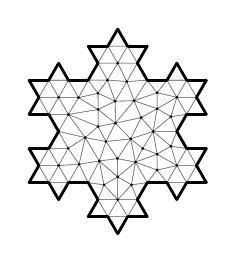
\begin{tikzpicture}[scale=1.3,baseline]   \draw[gray,very thin] (0.346410,0.000000) -- (0.519615,0.144444) -- (0.384900,0.222222) -- (0.346410,0.000000) ;
  \draw[gray,very thin] (-0.024755,0.295315) -- (-0.023014,0.080772) -- (0.160375,0.300000) -- (-0.024755,0.295315) ;
  \draw[gray,very thin] (-0.577350,-0.333333) -- (-0.673575,-0.500000) -- (-0.481125,-0.500000) -- (-0.577350,-0.333333) ;
  \draw[gray,very thin] (-0.866025,-0.500000) -- (-0.673575,-0.500000) -- (-0.769800,-0.333333) -- (-0.866025,-0.500000) ;
  \draw[gray,very thin] (-0.866025,-0.166667) -- (-0.769800,-0.333333) -- (-0.673575,-0.166667) -- (-0.866025,-0.166667) ;
  \draw[gray,very thin] (0.173205,-0.300000) -- (0.000000,-0.444444) -- (0.134715,-0.522222) -- (0.173205,-0.300000) ;
  \draw[gray,very thin] (-0.769800,-0.333333) -- (-0.673575,-0.500000) -- (-0.577350,-0.333333) -- (-0.769800,-0.333333) ;
  \draw[gray,very thin] (0.577350,0.000000) -- (0.673575,0.166667) -- (0.519615,0.144444) -- (0.577350,0.000000) ;
  \draw[gray,very thin] (-0.673575,-0.500000) -- (-0.577350,-0.666667) -- (-0.481125,-0.500000) -- (-0.673575,-0.500000) ;
  \draw[gray,very thin] (0.160375,0.300000) -- (0.384900,0.377778) -- (0.288675,0.500000) -- (0.160375,0.300000) ;
  \draw[gray,very thin] (-0.179620,-0.288889) -- (-0.134715,-0.522222) -- (0.000000,-0.444444) -- (-0.179620,-0.288889) ;
  \draw[gray,very thin] (0.577350,0.333333) -- (0.519615,0.144444) -- (0.673575,0.166667) -- (0.577350,0.333333) ;
  \draw[gray,very thin] (-0.192450,-0.666667) -- (-0.096225,-0.833333) -- (0.000000,-0.666667) -- (-0.192450,-0.666667) ;
  \draw[gray,very thin] (-0.288675,-0.833333) -- (-0.096225,-0.833333) -- (-0.192450,-0.666667) -- (-0.288675,-0.833333) ;
  \draw[gray,very thin] (0.192450,0.666667) -- (0.000000,0.666667) -- (0.088770,0.487087) -- (0.192450,0.666667) ;
  \draw[gray,very thin] (-0.484564,-0.164681) -- (-0.577350,0.000000) -- (-0.673575,-0.166667) -- (-0.484564,-0.164681) ;
  \draw[gray,very thin] (-0.288675,-0.500000) -- (-0.192450,-0.666667) -- (-0.134715,-0.522222) -- (-0.288675,-0.500000) ;
  \draw[gray,very thin] (-0.769800,-0.333333) -- (-0.577350,-0.333333) -- (-0.673575,-0.166667) -- (-0.769800,-0.333333) ;
  \draw[gray,very thin] (0.000000,-0.666667) -- (-0.096225,-0.833333) -- (0.096225,-0.833333) -- (0.000000,-0.666667) ;
  \draw[gray,very thin] (0.000000,-0.666667) -- (-0.134715,-0.522222) -- (-0.192450,-0.666667) -- (0.000000,-0.666667) ;
  \draw[gray,very thin] (0.384900,0.222222) -- (0.228882,0.134801) -- (0.346410,0.000000) -- (0.384900,0.222222) ;
  \draw[gray,very thin] (-0.377445,-0.320420) -- (-0.577350,-0.333333) -- (-0.481125,-0.500000) -- (-0.377445,-0.320420) ;
  \draw[gray,very thin] (0.173205,-0.300000) -- (0.134715,-0.522222) -- (0.288675,-0.500000) -- (0.173205,-0.300000) ;
  \draw[gray,very thin] (-0.002300,-0.265618) -- (0.173205,-0.300000) -- (0.126543,-0.073060) -- (-0.002300,-0.265618) ;
  \draw[gray,very thin] (-0.769800,0.333333) -- (-0.673575,0.166667) -- (-0.577350,0.333333) -- (-0.769800,0.333333) ;
  \draw[gray,very thin] (-0.866025,0.166667) -- (-0.673575,0.166667) -- (-0.769800,0.333333) -- (-0.866025,0.166667) ;
  \draw[gray,very thin] (-0.866025,0.500000) -- (-0.769800,0.333333) -- (-0.673575,0.500000) -- (-0.866025,0.500000) ;
  \draw[gray,very thin] (0.288675,-0.500000) -- (0.384900,-0.377778) -- (0.173205,-0.300000) -- (0.288675,-0.500000) ;
  \draw[gray,very thin] (-0.673575,0.500000) -- (-0.769800,0.333333) -- (-0.577350,0.333333) -- (-0.673575,0.500000) ;
  \draw[gray,very thin] (0.000000,-0.666667) -- (0.134715,-0.522222) -- (0.000000,-0.444444) -- (0.000000,-0.666667) ;
  \draw[gray,very thin] (-0.481125,0.500000) -- (-0.673575,0.500000) -- (-0.577350,0.333333) -- (-0.481125,0.500000) ;
  \draw[gray,very thin] (-0.482235,0.166026) -- (-0.317460,-0.060428) -- (-0.192007,0.048135) -- (-0.482235,0.166026) ;
  \draw[gray,very thin] (0.384900,-0.377778) -- (0.577350,-0.333333) -- (0.384900,-0.222222) -- (0.384900,-0.377778) ;
  \draw[gray,very thin] (-0.481125,0.500000) -- (-0.577350,0.666667) -- (-0.673575,0.500000) -- (-0.481125,0.500000) ;
  \draw[gray,very thin] (-0.577350,0.333333) -- (-0.382627,0.329396) -- (-0.481125,0.500000) -- (-0.577350,0.333333) ;
  \draw[gray,very thin] (-0.577350,0.000000) -- (-0.482235,0.166026) -- (-0.673575,0.166667) -- (-0.577350,0.000000) ;
  \draw[gray,very thin] (-0.288675,0.833333) -- (-0.192450,0.666667) -- (-0.096225,0.833333) -- (-0.288675,0.833333) ;
  \draw[gray,very thin] (-0.377445,-0.320420) -- (-0.481125,-0.500000) -- (-0.288675,-0.500000) -- (-0.377445,-0.320420) ;
  \draw[gray,very thin] (-0.096225,0.833333) -- (-0.192450,0.666667) -- (0.000000,0.666667) -- (-0.096225,0.833333) ;
  \draw[gray,very thin] (0.519615,-0.144444) -- (0.577350,-0.333333) -- (0.673575,-0.166667) -- (0.519615,-0.144444) ;
  \draw[gray,very thin] (-0.179620,-0.288889) -- (-0.288675,-0.500000) -- (-0.134715,-0.522222) -- (-0.179620,-0.288889) ;
  \draw[gray,very thin] (0.346410,0.000000) -- (0.384900,-0.222222) -- (0.519615,-0.144444) -- (0.346410,0.000000) ;
  \draw[gray,very thin] (-0.099664,0.501985) -- (-0.192826,0.373078) -- (-0.024755,0.295315) -- (-0.099664,0.501985) ;
  \draw[gray,very thin] (0.384900,0.222222) -- (0.160375,0.300000) -- (0.228882,0.134801) -- (0.384900,0.222222) ;
  \draw[gray,very thin] (-0.096225,-0.833333) -- (0.000000,-1.000000) -- (0.096225,-0.833333) -- (-0.096225,-0.833333) ;
  \draw[gray,very thin] (0.577350,0.333333) -- (0.384900,0.377778) -- (0.384900,0.222222) -- (0.577350,0.333333) ;
  \draw[gray,very thin] (0.096225,-0.833333) -- (0.288675,-0.833333) -- (0.192450,-0.666667) -- (0.096225,-0.833333) ;
  \draw[gray,very thin] (-0.134715,-0.522222) -- (0.000000,-0.666667) -- (0.000000,-0.444444) -- (-0.134715,-0.522222) ;
  \draw[gray,very thin] (0.288675,-0.500000) -- (0.481125,-0.500000) -- (0.384900,-0.377778) -- (0.288675,-0.500000) ;
  \draw[gray,very thin] (0.192450,-0.666667) -- (0.288675,-0.500000) -- (0.134715,-0.522222) -- (0.192450,-0.666667) ;
  \draw[gray,very thin] (-0.099664,0.501985) -- (-0.192450,0.666667) -- (-0.288675,0.500000) -- (-0.099664,0.501985) ;
  \draw[gray,very thin] (0.134715,-0.522222) -- (0.000000,-0.666667) -- (0.192450,-0.666667) -- (0.134715,-0.522222) ;
  \draw[gray,very thin] (0.481125,-0.500000) -- (0.577350,-0.666667) -- (0.673575,-0.500000) -- (0.481125,-0.500000) ;
  \draw[gray,very thin] (0.481125,-0.500000) -- (0.673575,-0.500000) -- (0.577350,-0.333333) -- (0.481125,-0.500000) ;
  \draw[gray,very thin] (0.346410,0.000000) -- (0.126543,-0.073060) -- (0.244503,-0.167073) -- (0.346410,0.000000) ;
  \draw[gray,very thin] (-0.114417,-0.098508) -- (0.126543,-0.073060) -- (-0.023014,0.080772) -- (-0.114417,-0.098508) ;
  \draw[gray,very thin] (0.673575,-0.500000) -- (0.866025,-0.500000) -- (0.769800,-0.333333) -- (0.673575,-0.500000) ;
  \draw[gray,very thin] (0.384900,0.377778) -- (0.160375,0.300000) -- (0.384900,0.222222) -- (0.384900,0.377778) ;
  \draw[gray,very thin] (0.577350,-0.333333) -- (0.519615,-0.144444) -- (0.384900,-0.222222) -- (0.577350,-0.333333) ;
  \draw[gray,very thin] (0.673575,-0.166667) -- (0.577350,-0.333333) -- (0.769800,-0.333333) -- (0.673575,-0.166667) ;
  \draw[gray,very thin] (0.519615,0.144444) -- (0.577350,0.333333) -- (0.384900,0.222222) -- (0.519615,0.144444) ;
  \draw[gray,very thin] (0.519615,-0.144444) -- (0.673575,-0.166667) -- (0.577350,0.000000) -- (0.519615,-0.144444) ;
  \draw[gray,very thin] (0.866025,-0.166667) -- (0.673575,-0.166667) -- (0.769800,-0.333333) -- (0.866025,-0.166667) ;
  \draw[gray,very thin] (0.577350,0.000000) -- (0.519615,0.144444) -- (0.346410,0.000000) -- (0.577350,0.000000) ;
  \draw[gray,very thin] (-0.317460,-0.060428) -- (-0.484564,-0.164681) -- (-0.377445,-0.320420) -- (-0.317460,-0.060428) ;
  \draw[gray,very thin] (0.673575,-0.500000) -- (0.769800,-0.333333) -- (0.577350,-0.333333) -- (0.673575,-0.500000) ;
  \draw[gray,very thin] (0.173205,-0.300000) -- (0.384900,-0.222222) -- (0.244503,-0.167073) -- (0.173205,-0.300000) ;
  \draw[gray,very thin] (-0.317460,-0.060428) -- (-0.577350,0.000000) -- (-0.484564,-0.164681) -- (-0.317460,-0.060428) ;
  \draw[gray,very thin] (-0.577350,-0.333333) -- (-0.377445,-0.320420) -- (-0.484564,-0.164681) -- (-0.577350,-0.333333) ;
  \draw[gray,very thin] (0.000000,0.666667) -- (0.192450,0.666667) -- (0.096225,0.833333) -- (0.000000,0.666667) ;
  \draw[gray,very thin] (0.384900,0.377778) -- (0.481125,0.500000) -- (0.288675,0.500000) -- (0.384900,0.377778) ;
  \draw[gray,very thin] (-0.191155,0.214038) -- (-0.382627,0.329396) -- (-0.482235,0.166026) -- (-0.191155,0.214038) ;
  \draw[gray,very thin] (0.346410,0.000000) -- (0.519615,-0.144444) -- (0.577350,0.000000) -- (0.346410,0.000000) ;
  \draw[gray,very thin] (-0.096225,0.833333) -- (0.096225,0.833333) -- (0.000000,1.000000) -- (-0.096225,0.833333) ;
  \draw[gray,very thin] (0.288675,0.833333) -- (0.096225,0.833333) -- (0.192450,0.666667) -- (0.288675,0.833333) ;
  \draw[gray,very thin] (0.000000,-0.444444) -- (0.173205,-0.300000) -- (-0.002300,-0.265618) -- (0.000000,-0.444444) ;
  \draw[gray,very thin] (0.288675,0.500000) -- (0.088770,0.487087) -- (0.160375,0.300000) -- (0.288675,0.500000) ;
  \draw[gray,very thin] (0.000000,0.666667) -- (0.096225,0.833333) -- (-0.096225,0.833333) -- (0.000000,0.666667) ;
  \draw[gray,very thin] (0.673575,0.166667) -- (0.866025,0.166667) -- (0.769800,0.333333) -- (0.673575,0.166667) ;
  \draw[gray,very thin] (0.384900,0.377778) -- (0.577350,0.333333) -- (0.481125,0.500000) -- (0.384900,0.377778) ;
  \draw[gray,very thin] (0.173205,-0.300000) -- (0.384900,-0.377778) -- (0.384900,-0.222222) -- (0.173205,-0.300000) ;
  \draw[gray,very thin] (0.673575,0.500000) -- (0.481125,0.500000) -- (0.577350,0.333333) -- (0.673575,0.500000) ;
  \draw[gray,very thin] (0.577350,-0.333333) -- (0.384900,-0.377778) -- (0.481125,-0.500000) -- (0.577350,-0.333333) ;
  \draw[gray,very thin] (0.577350,0.666667) -- (0.481125,0.500000) -- (0.673575,0.500000) -- (0.577350,0.666667) ;
  \draw[gray,very thin] (0.866025,0.500000) -- (0.673575,0.500000) -- (0.769800,0.333333) -- (0.866025,0.500000) ;
  \draw[gray,very thin] (-0.002300,-0.265618) -- (-0.179620,-0.288889) -- (0.000000,-0.444444) -- (-0.002300,-0.265618) ;
  \draw[gray,very thin] (-0.192826,0.373078) -- (-0.099664,0.501985) -- (-0.288675,0.500000) -- (-0.192826,0.373078) ;
  \draw[gray,very thin] (0.769800,0.333333) -- (0.673575,0.500000) -- (0.577350,0.333333) -- (0.769800,0.333333) ;
  \draw[gray,very thin] (0.769800,0.333333) -- (0.577350,0.333333) -- (0.673575,0.166667) -- (0.769800,0.333333) ;
  \draw[gray,very thin] (-0.377445,-0.320420) -- (-0.179620,-0.288889) -- (-0.317460,-0.060428) -- (-0.377445,-0.320420) ;
  \draw[gray,very thin] (-0.577350,-0.333333) -- (-0.484564,-0.164681) -- (-0.673575,-0.166667) -- (-0.577350,-0.333333) ;
  \draw[gray,very thin] (0.192450,-0.666667) -- (0.000000,-0.666667) -- (0.096225,-0.833333) -- (0.192450,-0.666667) ;
  \draw[gray,very thin] (0.126543,-0.073060) -- (-0.114417,-0.098508) -- (-0.002300,-0.265618) -- (0.126543,-0.073060) ;
  \draw[gray,very thin] (-0.288675,-0.500000) -- (-0.179620,-0.288889) -- (-0.377445,-0.320420) -- (-0.288675,-0.500000) ;
  \draw[gray,very thin] (0.192450,0.666667) -- (0.088770,0.487087) -- (0.288675,0.500000) -- (0.192450,0.666667) ;
  \draw[gray,very thin] (0.000000,0.666667) -- (-0.192450,0.666667) -- (-0.099664,0.501985) -- (0.000000,0.666667) ;
  \draw[gray,very thin] (-0.192826,0.373078) -- (-0.288675,0.500000) -- (-0.382627,0.329396) -- (-0.192826,0.373078) ;
  \draw[gray,very thin] (0.000000,0.666667) -- (-0.099664,0.501985) -- (0.088770,0.487087) -- (0.000000,0.666667) ;
  \draw[gray,very thin] (-0.002300,-0.265618) -- (-0.114417,-0.098508) -- (-0.179620,-0.288889) -- (-0.002300,-0.265618) ;
  \draw[gray,very thin] (0.088770,0.487087) -- (-0.099664,0.501985) -- (-0.024755,0.295315) -- (0.088770,0.487087) ;
  \draw[gray,very thin] (-0.288675,0.500000) -- (-0.481125,0.500000) -- (-0.382627,0.329396) -- (-0.288675,0.500000) ;
  \draw[gray,very thin] (-0.024755,0.295315) -- (-0.192826,0.373078) -- (-0.191155,0.214038) -- (-0.024755,0.295315) ;
  \draw[gray,very thin] (-0.577350,0.333333) -- (-0.673575,0.166667) -- (-0.482235,0.166026) -- (-0.577350,0.333333) ;
  \draw[gray,very thin] (-0.191155,0.214038) -- (-0.192826,0.373078) -- (-0.382627,0.329396) -- (-0.191155,0.214038) ;
  \draw[gray,very thin] (-0.023014,0.080772) -- (-0.024755,0.295315) -- (-0.191155,0.214038) -- (-0.023014,0.080772) ;
  \draw[gray,very thin] (0.088770,0.487087) -- (-0.024755,0.295315) -- (0.160375,0.300000) -- (0.088770,0.487087) ;
  \draw[gray,very thin] (-0.317460,-0.060428) -- (-0.482235,0.166026) -- (-0.577350,0.000000) -- (-0.317460,-0.060428) ;
  \draw[gray,very thin] (-0.577350,0.333333) -- (-0.482235,0.166026) -- (-0.382627,0.329396) -- (-0.577350,0.333333) ;
  \draw[gray,very thin] (-0.191155,0.214038) -- (-0.482235,0.166026) -- (-0.192007,0.048135) -- (-0.191155,0.214038) ;
  \draw[gray,very thin] (-0.023014,0.080772) -- (0.126543,-0.073060) -- (0.228882,0.134801) -- (-0.023014,0.080772) ;
  \draw[gray,very thin] (-0.192007,0.048135) -- (-0.023014,0.080772) -- (-0.191155,0.214038) -- (-0.192007,0.048135) ;
  \draw[gray,very thin] (-0.317460,-0.060428) -- (-0.179620,-0.288889) -- (-0.114417,-0.098508) -- (-0.317460,-0.060428) ;
  \draw[gray,very thin] (-0.317460,-0.060428) -- (-0.114417,-0.098508) -- (-0.192007,0.048135) -- (-0.317460,-0.060428) ;
  \draw[gray,very thin] (-0.023014,0.080772) -- (-0.192007,0.048135) -- (-0.114417,-0.098508) -- (-0.023014,0.080772) ;
  \draw[gray,very thin] (-0.023014,0.080772) -- (0.228882,0.134801) -- (0.160375,0.300000) -- (-0.023014,0.080772) ;
  \draw[gray,very thin] (0.126543,-0.073060) -- (0.346410,0.000000) -- (0.228882,0.134801) -- (0.126543,-0.073060) ;
  \draw[gray,very thin] (0.346410,0.000000) -- (0.244503,-0.167073) -- (0.384900,-0.222222) -- (0.346410,0.000000) ;
  \draw[gray,very thin] (0.126543,-0.073060) -- (0.173205,-0.300000) -- (0.244503,-0.167073) -- (0.126543,-0.073060) ;
  \filldraw (-0.866025,0.500000) circle (0.200000pt);
  \filldraw (-0.673575,0.500000) circle (0.200000pt);
  \filldraw (-0.577350,0.666667) circle (0.200000pt);
  \filldraw (-0.481125,0.500000) circle (0.200000pt);
  \filldraw (-0.288675,0.500000) circle (0.200000pt);
  \filldraw (-0.192450,0.666667) circle (0.200000pt);
  \filldraw (-0.288675,0.833333) circle (0.200000pt);
  \filldraw (-0.096225,0.833333) circle (0.200000pt);
  \filldraw (0.000000,1.000000) circle (0.200000pt);
  \filldraw (0.096225,0.833333) circle (0.200000pt);
  \filldraw (0.288675,0.833333) circle (0.200000pt);
  \filldraw (0.192450,0.666667) circle (0.200000pt);
  \filldraw (0.288675,0.500000) circle (0.200000pt);
  \filldraw (0.481125,0.500000) circle (0.200000pt);
  \filldraw (0.577350,0.666667) circle (0.200000pt);
  \filldraw (0.673575,0.500000) circle (0.200000pt);
  \filldraw (0.866025,0.500000) circle (0.200000pt);
  \filldraw (0.769800,0.333333) circle (0.200000pt);
  \filldraw (0.866025,0.166667) circle (0.200000pt);
  \filldraw (0.673575,0.166667) circle (0.200000pt);
  \filldraw (0.577350,0.000000) circle (0.200000pt);
  \filldraw (0.673575,-0.166667) circle (0.200000pt);
  \filldraw (0.866025,-0.166667) circle (0.200000pt);
  \filldraw (0.769800,-0.333333) circle (0.200000pt);
  \filldraw (0.866025,-0.500000) circle (0.200000pt);
  \filldraw (0.673575,-0.500000) circle (0.200000pt);
  \filldraw (0.577350,-0.666667) circle (0.200000pt);
  \filldraw (0.481125,-0.500000) circle (0.200000pt);
  \filldraw (0.288675,-0.500000) circle (0.200000pt);
  \filldraw (0.192450,-0.666667) circle (0.200000pt);
  \filldraw (0.288675,-0.833333) circle (0.200000pt);
  \filldraw (0.096225,-0.833333) circle (0.200000pt);
  \filldraw (0.000000,-1.000000) circle (0.200000pt);
  \filldraw (-0.096225,-0.833333) circle (0.200000pt);
  \filldraw (-0.288675,-0.833333) circle (0.200000pt);
  \filldraw (-0.192450,-0.666667) circle (0.200000pt);
  \filldraw (-0.288675,-0.500000) circle (0.200000pt);
  \filldraw (-0.481125,-0.500000) circle (0.200000pt);
  \filldraw (-0.577350,-0.666667) circle (0.200000pt);
  \filldraw (-0.673575,-0.500000) circle (0.200000pt);
  \filldraw (-0.866025,-0.500000) circle (0.200000pt);
  \filldraw (-0.769800,-0.333333) circle (0.200000pt);
  \filldraw (-0.866025,-0.166667) circle (0.200000pt);
  \filldraw (-0.673575,-0.166667) circle (0.200000pt);
  \filldraw (-0.577350,0.000000) circle (0.200000pt);
  \filldraw (-0.673575,0.166667) circle (0.200000pt);
  \filldraw (-0.866025,0.166667) circle (0.200000pt);
  \filldraw (-0.769800,0.333333) circle (0.200000pt);
  \filldraw (-0.577350,-0.333333) circle (0.200000pt);
  \filldraw (0.000000,-0.444444) circle (0.200000pt);
  \filldraw (-0.577350,0.333333) circle (0.200000pt);
  \filldraw (0.000000,0.666667) circle (0.200000pt);
  \filldraw (0.384900,-0.222222) circle (0.200000pt);
  \filldraw (0.577350,-0.333333) circle (0.200000pt);
  \filldraw (0.384900,0.222222) circle (0.200000pt);
  \filldraw (0.577350,0.333333) circle (0.200000pt);
  \filldraw (0.000000,-0.666667) circle (0.200000pt);
  \filldraw (-0.134715,-0.522222) circle (0.200000pt);
  \filldraw (-0.179620,-0.288889) circle (0.200000pt);
  \filldraw (0.134715,-0.522222) circle (0.200000pt);
  \filldraw (0.173205,-0.300000) circle (0.200000pt);
  \filldraw (0.384900,-0.377778) circle (0.200000pt);
  \filldraw (0.519615,-0.144444) circle (0.200000pt);
  \filldraw (0.346410,0.000000) circle (0.200000pt);
  \filldraw (0.519615,0.144444) circle (0.200000pt);
  \filldraw (0.384900,0.377778) circle (0.200000pt);
  \filldraw (0.160375,0.300000) circle (0.200000pt);
  \filldraw (-0.377445,-0.320420) circle (0.200000pt);
  \filldraw (-0.317460,-0.060428) circle (0.200000pt);
  \filldraw (-0.484564,-0.164681) circle (0.200000pt);
  \filldraw (-0.002300,-0.265618) circle (0.200000pt);
  \filldraw (0.126543,-0.073060) circle (0.200000pt);
  \filldraw (0.088770,0.487087) circle (0.200000pt);
  \filldraw (-0.099664,0.501985) circle (0.200000pt);
  \filldraw (-0.191155,0.214038) circle (0.200000pt);
  \filldraw (-0.192826,0.373078) circle (0.200000pt);
  \filldraw (-0.382627,0.329396) circle (0.200000pt);
  \filldraw (-0.024755,0.295315) circle (0.200000pt);
  \filldraw (-0.482235,0.166026) circle (0.200000pt);
  \filldraw (-0.023014,0.080772) circle (0.200000pt);
  \filldraw (-0.114417,-0.098508) circle (0.200000pt);
  \filldraw (-0.192007,0.048135) circle (0.200000pt);
  \filldraw (0.228882,0.134801) circle (0.200000pt);
  \filldraw (0.244503,-0.167073) circle (0.200000pt);
  \draw[line width=1.000000pt] (-0.673575,0.500000) -- (-0.866025,0.500000);
  \draw[line width=1.000000pt] (-0.673575,0.500000) -- (-0.577350,0.666667);
  \draw[line width=1.000000pt] (-0.481125,0.500000) -- (-0.577350,0.666667);
  \draw[line width=1.000000pt] (-0.288675,0.500000) -- (-0.481125,0.500000);
  \draw[line width=1.000000pt] (-0.288675,0.500000) -- (-0.192450,0.666667);
  \draw[line width=1.000000pt] (-0.192450,0.666667) -- (-0.288675,0.833333);
  \draw[line width=1.000000pt] (-0.288675,0.833333) -- (-0.096225,0.833333);
  \draw[line width=1.000000pt] (-0.096225,0.833333) -- (0.000000,1.000000);
  \draw[line width=1.000000pt] (0.096225,0.833333) -- (0.000000,1.000000);
  \draw[line width=1.000000pt] (0.096225,0.833333) -- (0.288675,0.833333);
  \draw[line width=1.000000pt] (0.192450,0.666667) -- (0.288675,0.833333);
  \draw[line width=1.000000pt] (0.192450,0.666667) -- (0.288675,0.500000);
  \draw[line width=1.000000pt] (0.481125,0.500000) -- (0.288675,0.500000);
  \draw[line width=1.000000pt] (0.481125,0.500000) -- (0.577350,0.666667);
  \draw[line width=1.000000pt] (0.577350,0.666667) -- (0.673575,0.500000);
  \draw[line width=1.000000pt] (0.673575,0.500000) -- (0.866025,0.500000);
  \draw[line width=1.000000pt] (0.866025,0.500000) -- (0.769800,0.333333);
  \draw[line width=1.000000pt] (0.769800,0.333333) -- (0.866025,0.166667);
  \draw[line width=1.000000pt] (0.866025,0.166667) -- (0.673575,0.166667);
  \draw[line width=1.000000pt] (0.673575,0.166667) -- (0.577350,0.000000);
  \draw[line width=1.000000pt] (0.673575,-0.166667) -- (0.577350,0.000000);
  \draw[line width=1.000000pt] (0.673575,-0.166667) -- (0.866025,-0.166667);
  \draw[line width=1.000000pt] (0.866025,-0.166667) -- (0.769800,-0.333333);
  \draw[line width=1.000000pt] (0.769800,-0.333333) -- (0.866025,-0.500000);
  \draw[line width=1.000000pt] (0.866025,-0.500000) -- (0.673575,-0.500000);
  \draw[line width=1.000000pt] (0.673575,-0.500000) -- (0.577350,-0.666667);
  \draw[line width=1.000000pt] (0.577350,-0.666667) -- (0.481125,-0.500000);
  \draw[line width=1.000000pt] (0.481125,-0.500000) -- (0.288675,-0.500000);
  \draw[line width=1.000000pt] (0.288675,-0.500000) -- (0.192450,-0.666667);
  \draw[line width=1.000000pt] (0.192450,-0.666667) -- (0.288675,-0.833333);
  \draw[line width=1.000000pt] (0.288675,-0.833333) -- (0.096225,-0.833333);
  \draw[line width=1.000000pt] (0.096225,-0.833333) -- (0.000000,-1.000000);
  \draw[line width=1.000000pt] (0.000000,-1.000000) -- (-0.096225,-0.833333);
  \draw[line width=1.000000pt] (-0.288675,-0.833333) -- (-0.096225,-0.833333);
  \draw[line width=1.000000pt] (-0.192450,-0.666667) -- (-0.288675,-0.833333);
  \draw[line width=1.000000pt] (-0.192450,-0.666667) -- (-0.288675,-0.500000);
  \draw[line width=1.000000pt] (-0.481125,-0.500000) -- (-0.288675,-0.500000);
  \draw[line width=1.000000pt] (-0.481125,-0.500000) -- (-0.577350,-0.666667);
  \draw[line width=1.000000pt] (-0.577350,-0.666667) -- (-0.673575,-0.500000);
  \draw[line width=1.000000pt] (-0.866025,-0.500000) -- (-0.673575,-0.500000);
  \draw[line width=1.000000pt] (-0.769800,-0.333333) -- (-0.866025,-0.500000);
  \draw[line width=1.000000pt] (-0.769800,-0.333333) -- (-0.866025,-0.166667);
  \draw[line width=1.000000pt] (-0.673575,-0.166667) -- (-0.866025,-0.166667);
  \draw[line width=1.000000pt] (-0.673575,-0.166667) -- (-0.577350,0.000000);
  \draw[line width=1.000000pt] (-0.577350,0.000000) -- (-0.673575,0.166667);
  \draw[line width=1.000000pt] (-0.673575,0.166667) -- (-0.866025,0.166667);
  \draw[line width=1.000000pt] (-0.769800,0.333333) -- (-0.866025,0.166667);
  \draw[line width=1.000000pt] (-0.769800,0.333333) -- (-0.866025,0.500000);
 \end{tikzpicture}
\end{center}

\footnotesize
\item \alert{Fall 2018: graduate seminar in FEM}
\end{itemize}
\end{frame}


\begin{frame}{finite element method}

in more detail, the FEM uses
\begin{itemize}
\item a {\footnotesize triangular/quadrilateral/tetrahedral/etc.}~mesh of $N$ nodes $\bx_i$ on $\Omega$
\item an $N$-dimensional subspace $\mathcal{X} \subset H^1(\Omega)$ with basis $\{\psi_j\}$ of
\item \begin{minipage}[t]{55mm}
\dots \emph{hat functions} $\psi_j$
	\begin{itemize}
	\item[$\circ$] $\psi_j(\bx_i)=0$ except $\psi_j(\bx_j)=1$
	\end{itemize}
\end{minipage}
\quad
\begin{minipage}[t]{35mm}
\vspace{-4mm}
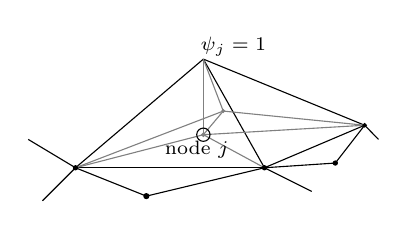
\begin{tikzpicture}[scale=0.6, z={(.707,.3)}, baseline]
    % (2,2,1) is top
    \draw (0,0,0) -- (2,2,1); % to top from left
    \draw (4,0,0) -- (2,2,1); %   ...  from front
    \draw (4,0,3) -- (2,2,1); %   ...  from right
    \draw[color=gray] (0.3,0,4) -- (2,2,1); % from back
    \draw[color=gray] (2,0.4,1) -- (2,2,1); % from middle

    % draw base
    \draw (0,0,0) -- (4,0,0);
    \draw (4,0,0) -- (4,0,3);
    \draw[color=gray] (0,0,0) -- (0.3,0,4);
    \draw[color=gray] (0.3,0,4) -- (4,0,3);
    \draw[color=gray] (0,0,0) -- (2,0.4,1);
    \draw[color=gray] (2,0.4,1) -- (4,0,3);
    \draw[color=gray] (4,0,0) -- (2,0.4,1);
    \draw[color=gray] (2,0.4,1) -- (0.3,0,4);

    % extend flat
    \draw (0,0,0) -- (-0.7,-0.7,0);
    \draw (0,0,0) -- (1.5,-0.6,0);
    \draw (0,0,0) -- (-1,0.6,0);
    \draw (4,0,0) -- (1.5,-0.6,0);
    \draw (4,0,0) -- (5.5,0.1,0);
    \draw (4,0,0) -- (5,-0.5,0);
    \draw (4,0,3) -- (5.5,0.1,0);
    \draw (4,0,3) -- (5,0,2);

    % label node j
    \draw (2,2,1.9) node {{\scriptsize $\psi_j=1$}};
    \draw (2,0.15,0.8) node {{\scriptsize node $j$}};
    \draw (2,0.4,1) circle (4.0pt);

    % draw nodes
    \filldraw[color=gray] (0.3,0,4) circle (0.8pt);
    \filldraw[color=gray] (2,0.4,1) circle (1.0pt);
    \filldraw (4,0,3) circle (1.0pt);
    \filldraw (0,0,0) circle (1.25pt);
    \filldraw (4,0,0) circle (1.25pt);
    \filldraw (5.5,0.1,0) circle (1.25pt);
    \filldraw (1.5,-0.6,0) circle (1.5pt);

\end{tikzpicture}
\end{minipage}
\end{itemize}

\vspace{-3mm}
then the FEM
\begin{itemize}
\item defines
   $$u(x,y) = \sum_j u_{j}\, \psi_{j}(x,y)$$
for unknown coefficients $\bu=\{u_j\}\in \RR^N$
\item and requires the weak form to hold for all $v=\psi_i$ ($N$ eqns)
\end{itemize}

\medskip
which again yields a system of $N$ eqns in $N$ unknowns
\end{frame}


\begin{frame}{linear systems with sparse matrices}
\begin{itemize}
\item both methods (\FM) produce \emph{sparse matrices}
\item for example, the Poisson equation becomes a linear system
    $$A \bu = \bb$$
    \vspace{-4mm}
	\begin{itemize}
	\item[$\circ$] $A\in\RR^{N\times N}$ is sparse
	\item[$\circ$] $A$ is symmetric positive definite (SPD)
	\end{itemize}
\item \emph{pro tip}: Matlab's \texttt{spy(A)} shows nonzero structure
\end{itemize}

\bigskip
\begin{center}
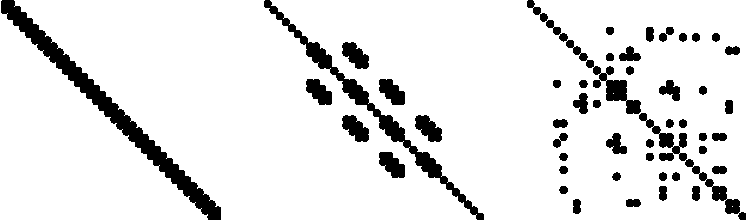
\includegraphics[width=0.85\textwidth]{figs/spythree}

\medskip
\scriptsize
Poisson 1D (either method) \quad MSE FDM 2D square \qquad Poisson FEM 2D snowflake

\end{center}
\end{frame}


\begin{frame}{nonlinear PDEs make sparse matrices too}
\begin{itemize}
\item \FM applied to a nonlinear elliptic PDE BVP gives a nonlinear (algebraic) system of $N$ equations in $N$ unknowns:
    $$\mathbf{F}(\bu)=0$$
     \vspace{-4mm}
	\begin{itemize}
	\item[$\circ$] $\mathbf{F}:\RR^N\to\RR^N$
	\item[$\circ$] $\mathbf{F}(\bw)$ is the \emph{residual} if $\bw$ is a guess at the solution
	\end{itemize}

\item \begin{minipage}[t]{70mm}
usually apply Newton's method to solve:
    $$J_{\mathbf{F}}(\bu_{\ell+1})\, \bs = - \mathbf{F}(\bu_\ell)$$
     \vspace{-4mm}
	\begin{itemize}
	\item[$\circ$] $J_{\mathbf{F}}(\bw) \in \RR^{N\times N}$ is the Jacobian of $\mathbf{F}$
	\item[$\circ$] $\bs \in \RR^N$ is the step
	\item[$\circ$] $A=J_{\mathbf{F}}(\bu_\ell)$ is a sparse matrix (right)
	\end{itemize}
\end{minipage}
\quad
\begin{minipage}[t]{20mm}
\vspace{0mm}
\hfill 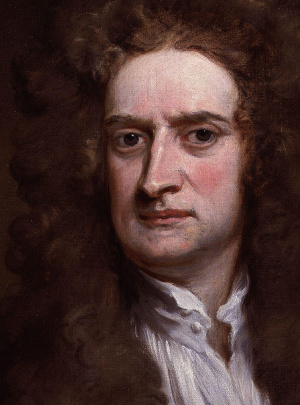
\includegraphics[width=0.6\textwidth]{figs/newton}

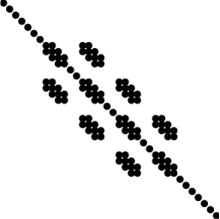
\includegraphics[width=\textwidth]{figs/spybanded}

\tiny
 MSE FDM 2D square
\end{minipage}
\end{itemize}
\end{frame}


\section{what is an ``optimal solver''?}

\begin{frame}{define ``optimal''}
\begin{itemize}
\item consider $N$ equations in $N$ unknowns: \qquad $\mathbf{F}(\mathbf{u}) = 0$
	\begin{itemize}
	\item[$\circ$] residual $\mathbf{F}:\RR^N \to \RR^N$ is generally nonlinear
	\item[$\circ$] $\mathbf{F}(\mathbf{w}) = \mathbf{b} - A \mathbf{w}$ in the linear case
	\end{itemize}

\bigskip\medskip
\noindent \textbf{definition.}  \begin{minipage}[t]{80mm}
an algorithm which solves $\mathbf{F}(\mathbf{u}) = 0$ in $O(N)$ work is \alert{\emph{optimal}}
\end{minipage}

\bigskip \bigskip
\item if you have ever tried solving big, nontrivially-coupled systems of equations, you'll conclude optimality is generally hopeless
\end{itemize}
\end{frame}


\begin{frame}{slide full of caveats}

in the definition ``an algorithm which solves $\mathbf{F}(\mathbf{u}) = 0$ in $O(N)$ work is \emph{optimal}'':
\begin{itemize}
\item  ``solves'' means that it generates $\mathbf{u}_n$ so that $\frac{\|\mathbf{F}(\mathbf{u}_n)\|}{\|\mathbf{F}(\mathbf{u}_0)\|} \le \text{tol}$ where $\mathbf{u}_0$ is an initial guess
	\begin{itemize}
	\item[$\circ$] in linear case $A\bu=\bb$, given any rounding error, only $O(\kappa(A)\eps_{\text{mach}})$ accuracy is possible anyway\footnote{for students of MATH 614}
    \item[$\circ$] ``$O(\dots)$'' hides a constant which may depend on tol but not on $N$
	\end{itemize}
\item ``work'' $=$ (count of floating point operations)
	\begin{itemize}
	\item[$\circ$] \emph{or} time for the algorithm to run, but timing on modern computers is really messy
	\end{itemize}
\item actually, $O(N\log N)$ is accepted as ``optimal'' too
\item a nearly-equivalent definition could say ``work is less than $O(N^{1+\delta})$ for any $\delta>0$''
\end{itemize}
\end{frame}


\begin{frame}{example: tridiagonal matrices}
\begin{itemize}
\item an easy example of optimality
\item Gauss elimination solves $A \bu = \bb$ in $8N-6=O(N)$ flops
	\begin{itemize}
	\item[$\circ$] need to avoid pivoting
	\end{itemize}
\item for SPD tridiagonal matrices, use \emph{banded Cholesky decomposition}, again $O(N)$
\item also applies to pentadiagonal, septadiagonal, \dots
\item the 1D Poisson problem $-u''=f$, and generally all ODE BVPs, have optimal solution methods
\end{itemize}

\bigskip
\begin{center}
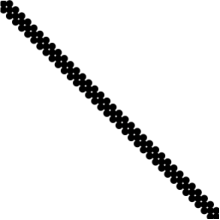
\includegraphics[width=0.2\textwidth]{figs/spytri}
\end{center}
\end{frame}


\begin{frame}{non-example:  banded direct methods in 2D,3D}
\begin{itemize}
\item for structured-grid FDM method on PDEs in 2D and 3D the bandwidth of $A$ grows as $h\to 0$
\item for example, for MSE on $\Omega=[0,1]\times[0,1]$:

\begin{center}
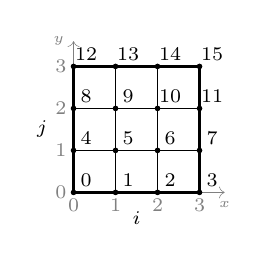
\begin{tikzpicture}[scale=1.6,baseline]   \draw[->,gray,very thin] (0.0,0.0) -- (1.2,0.0) node[below] {\tiny $x$};
  \draw[->,gray,very thin] (0.0,0.0) -- (0.0,1.2) node[left] {\tiny $y$};
  \draw[line width=1.0pt] (0.0,0.0) -- (0.0,1.0) -- (1.0,1.0) -- (1.0,0.0) -- cycle;
  \pgfmathsetmacro\third{1.0/3.0}
  \pgfmathsetmacro\half{1.0/2.0}
  \node[gray] at (0.0,-0.1) {\scriptsize $0$};
  \node[gray] at (\third,-0.1) {\scriptsize $1$};
  \node at (\half,-0.2) {\scriptsize $i$};
  \node[gray] at (2*\third,-0.1) {\scriptsize $2$};
  \node[gray] at (1.0,-0.1) {\scriptsize $3$};
  \node[gray] at (-0.1,0.0) {\scriptsize $0$};
  \node[gray] at (-0.1,\third) {\scriptsize $1$};
  \node[gray] at (-0.1,2*\third) {\scriptsize $2$};
  \node at (-0.25,0.5) {\scriptsize $j$};
  \node[gray] at (-0.1,1.0) {\scriptsize $3$};
  \draw[xstep=\third,ystep=\third,black,thin] (0.0,0.0) grid (1.0,1.0);
  \pgfmathsetmacro\dd{0.05}
  \foreach \y in {0,1,2,3} {
    \foreach \x in {0,1,2,3} {
      \pgfmathsetmacro\k{4*\y+\x}
  %    \draw (\x*\third+\dd,\y*\half+\dd) node{$\pgfmathprintnumber[fixed]{\k}$};
      \node at (\x * \third + 0.1,\y * \third + 0.1) {\scriptsize $\pgfmathprintnumber[fixed]{\k}$};
      \filldraw (\x * \third,\y * \third) circle (0.5pt);
    }
  }

 \end{tikzpicture} \qquad \begin{minipage}[b]{5mm} $\to$ \vspace{10mm} \end{minipage} \qquad 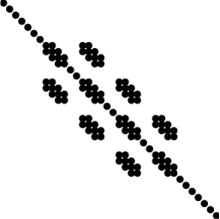
\includegraphics[width=0.19\textwidth]{figs/spybanded}
\end{center}

\item if $N\times N$ matrix $A$ has bandwidth $p$ then banded Cholesky does $O(N p^2)$ work
\item thus for direct methods for PDE problems on structured grids with $m$ points in each direction:
	\begin{itemize}
	\item[$\circ$] $N=m^2$ and $p=m$ so $O(N^2)$ work in 2D
	\item[$\circ$] $N=m^3$ and $p=m^2$ so $O(N^{7/3})$ work in 3D
	\end{itemize}
\item variable reordering helps a lot \dots but not enough
\end{itemize}
\end{frame}


\begin{frame}{sparse matrices from PDEs have $O(N)$ mat-vec}

\begin{itemize}
\item however, if
    \begin{itemize}
    \item[$\circ$] $A \in \RR^{N\times N}$ is sparse, and
    \item[$\circ$] number of nonzeros per row is bounded independent of $N$
    \end{itemize}
then the \emph{work of computing $A \bv$ is $O(N)$}
\item computing $A \bv$ is called a ``mat-vec''
\item the ``bounded'' condition is automatic for structured grids
\item for FEM on unstructured meshes
   $$\text{(nonzeros in row } j) = \operatorname{degree}(\text{node } j) + 1$$
so cost of $A\bv$ is $O((\max \operatorname{degree}) N)$
\end{itemize}

\smallskip
\begin{center}
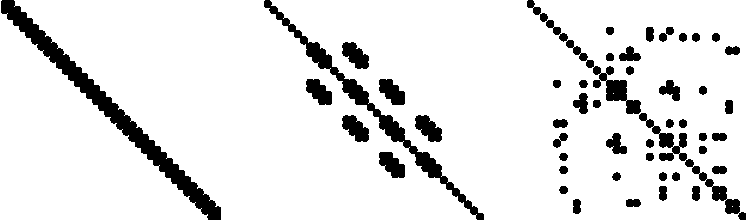
\includegraphics[width=0.65\textwidth]{figs/spythree}

\tiny

\qquad $3$ \qquad\qquad\qquad\qquad\qquad\qquad $9$ \quad\qquad\qquad\qquad\quad $\max \operatorname{degree} + 1$
\end{center}
\end{frame}


\begin{frame}{Krylov methods}
\begin{itemize}
\item among numerical analysts of the 1960s and 1970s, observing that sparse mat-vecs and residual evaluations are $O(N)$ for \FM discretizations was the new hope
\item \begin{minipage}[t]{0.7\textwidth}
naval engineer A.~Krylov (1931): the solution to $A\bu=\bb$ may be well-approximated by $\bv$ in

\vspace{-4mm}
$$\mathcal{K}_m(A,\bb) = \operatorname{span}\left\{\bb,A\bb,A^2\bb,\dots,A^m\bb\right\}$$
\end{minipage} \quad
\begin{minipage}[t]{0.18\textwidth}
\vspace{-3mm}

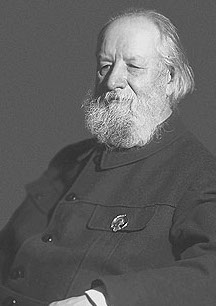
\includegraphics[width=\textwidth]{figs/krylov}
\end{minipage}

    \vspace{2mm}
	\begin{itemize}
	\item[$\circ$] computing $\bv \in \mathcal{K}_m(A,\bb)$ costs $O(mN)$
	\item[$\circ$] $\bv \in \mathcal{K}_m(A,\bb) \iff \bv = p_m(A) \bb$
	\end{itemize}
\item to solve $A\bu=\bb$ we want $\bu = A^{-1}\bb \approx p_m(A) \bb$
\end{itemize}
\end{frame}


\begin{frame}{conjugate gradients}

\begin{itemize}
\item example: \emph{conjugate gradients} (CG) is a Krylov method
	\begin{itemize}
	\item[$\circ$] $A$ must be SPD because CG is a minimization algorithm
	\item[$\circ$] CG generates the ``best'' iterates $\bv_m$ from a Krylov space
		\begin{itemize}
		\item the error $\be_m=\bv_m-\bu$ is minimal in norm $\|\cdot\|_A$
		\end{itemize}
	\item[$\circ$] work per iteration is $O(N)$ for $A$ from \FM
	\item[$\circ$] thus work is $O(mN)$ for $m$ iterations
	\end{itemize}
\item if $\kappa=\kappa_2(A)$ is the condition number of $A$ then
	$$\frac{\|\be_m\|_A}{\|\be_0\|_A} \le 2 \left(\frac{\sqrt{\kappa}-1}{\sqrt{\kappa}+1}\right)^m$$
\item it follows that $m = O(\sqrt{\kappa})$ iterations are needed
\end{itemize}
\end{frame}


\begin{frame}{CG iterations increase with $N$}

\begin{itemize}
\item unfortunately, if $A$ is from FDM applied to the Poisson equation then
    $$\kappa_2(A) = O(h^{-2})$$
\item \begin{minipage}[t]{55mm}
the number of CG iterations $m$ increases with $N=O(h^{-d})$
	\begin{itemize}
	\item[$\circ$] $m=O(N^{1/2})$ in 2D $\implies O(N^{3/2})$ solver
	\item[$\circ$] $m=O(N^{1/3})$ in 3D $\implies O(N^{4/3})$ solver
	\end{itemize}
\end{minipage} \quad
\begin{minipage}[t]{40mm}
\vspace{-2mm}

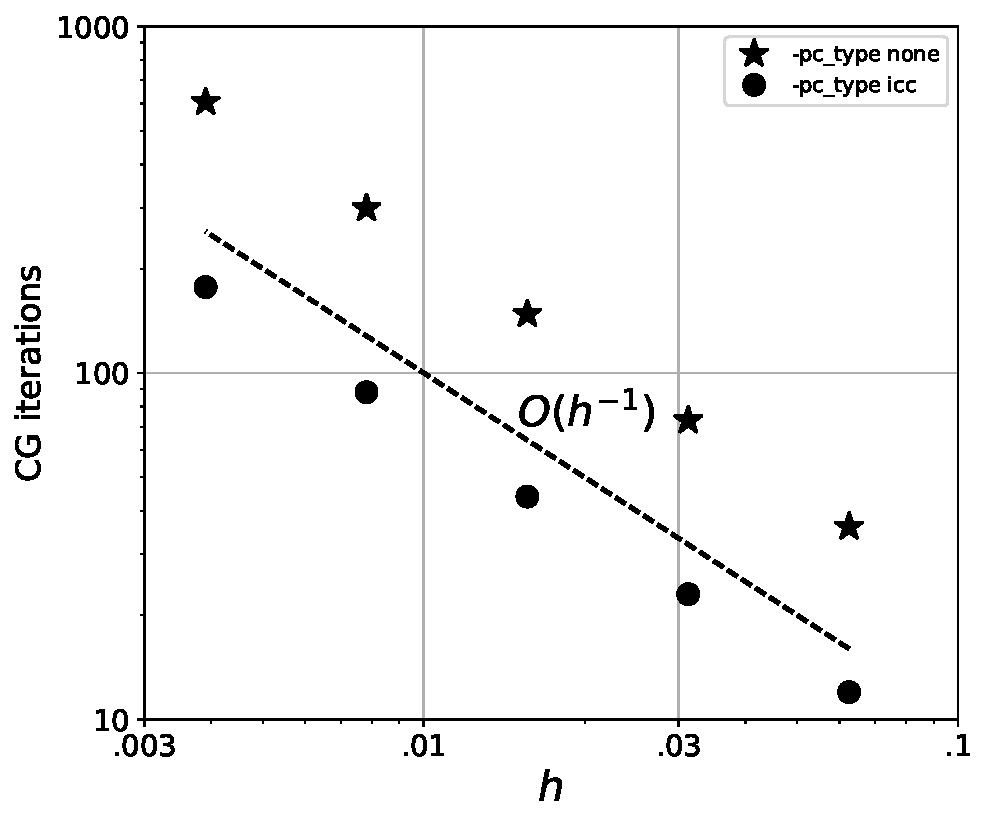
\includegraphics[width=\textwidth]{figs/poisson-cg-scale}
\end{minipage}

\vspace{-2mm}
\item other Krylov methods are similar

\vspace{5mm}
\item general lesson:

\begin{quote}
\alert{a Krylov method can only be optimal if the number of iterations $m$ is independent of $N$}
\end{quote}
\end{itemize}
\end{frame}


\begin{frame}{preconditioning}
\begin{itemize}
\item by $\sim$1995 it was clear that Krylov methods by themselves were not the answer for solving big PDE problems
\item but you don't have to accept the given system $A\bu=\bb$
\item \emph{definition}. given invertible $M$,
	\begin{itemize}
	\item[$\circ$] $(M^{-1}A)\bu=M^{-1}\bb$ is the \emph{left-preconditioned} system
	\item[$\circ$] $(AM^{-1})M\bu=\bb$ is the \emph{right-preconditioned} system
	\end{itemize}
\item new condition numbers $\kappa_2(M^{-1}A)$ or $\kappa_2(AM^{-1})$ can be much smaller
\item ``$M^{-1}$'' must be a cheap $O(N)$ method for this to help
	\begin{itemize}
	\item[$\circ$] e.g.~Meijerink \& van der Vorst (1977): incomplete LU and Cholesky factorizations
	\end{itemize}
\end{itemize}
\end{frame}


\begin{frame}{an optimality lemma}


\begin{itemize}
\item \emph{lemma}.  for SPD matrices $A\in\RR^{N\times N}$, if a symmetric preconditioning method produces bounded condition numbers,
     $$\kappa_2(M^{-1}A) \le B,$$
where $B>0$ is independent of $N$, then preconditioned CG is an optimal solver

    \medskip
	\begin{itemize}
	\item[$\circ$] or for right-preconditioning with ``$\kappa_2(AM^{-1})$''
	\end{itemize}

\vspace{5mm}
\item \emph{new goal}:  find preconditioners which make the new condition number $\kappa_2(M^{-1}A)$ bounded independent of $N$

\bigskip
\item \emph{multigrid} is such a preconditioner
\end{itemize}
\end{frame}


\section{multigrid}

\begin{frame}{multigrid: what it does}

\small
\begin{itemize}
\item given sequence of grids $\left\{\Omega^{(j)}\right\}_0^k$ \qquad \begin{tikzpicture}[scale=0.8,baseline]
\begin{tikzpicture}[scale=1.6]
  \pgfmathsetmacro\half{1.0/2.0}
  \draw[xstep=\half,ystep=\half,black,thin] (0.0,0.0) grid (1.0,1.0);
  \node at (0.5,-0.25) {$\Omega^{(0)}$};
\end{tikzpicture}
\quad
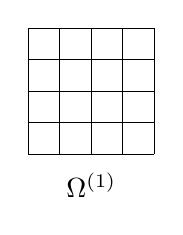
\begin{tikzpicture}[scale=1.6]
  \pgfmathsetmacro\fourth{1.0/4.0}
  \draw[xstep=\fourth,ystep=\fourth,black,thin] (0.0,0.0) grid (1.0,1.0);
  \node at (0.5,-0.25) {$\Omega^{(1)}$};
\end{tikzpicture}
\quad
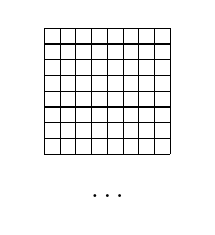
\begin{tikzpicture}[scale=1.6]
  \pgfmathsetmacro\eigth{1.0/8.0}
  \draw[xstep=\eigth,ystep=\eigth,black,thin] (0.0,0.0) grid (1.0,1.0);
  \node at (0.5,-0.25) {$\phantom{\Omega^{(2)}}\dots\phantom{\Omega^{(2)}}$};
\end{tikzpicture}
\quad
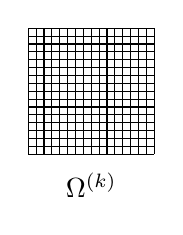
\begin{tikzpicture}[scale=1.6]
  \pgfmathsetmacro\sixteenth{1.0/16.0}
  \draw[xstep=\sixteenth,ystep=\sixteenth,black,thin] (0.0,0.0) grid (1.0,1.0);
  \node at (0.5,-0.25) {$\Omega^{(k)}$};
\end{tikzpicture}

\end{tikzpicture}
\item given initial guess $\bw$ on the finest grid $\Omega^{(k)}$
\item a multigrid cycle approximately solves $A \bu = \bb$
\item for example: $\bw \gets \text{\textsc{Vcycle}}(A,\bb,\bw,k)$
\end{itemize}

\begin{minipage}[t]{75mm}
\begin{algorithmic}
\footnotesize
\Function{Vcycle}{$A,\bb,\bw,l$}
    \If{$l == 0$}
        \State solve $A \bv = \bb$, e.g.~by a direct solver
    \Else
        \State improve $\bw$ on the level $l$ grid, giving $\bv$
        \State $\br^C = \left(\text{restrict } \br = \bb - A \bv \text{ to } \Omega^{(l-1)}\right)$
        \State $\bz^C = \text{\textsc{Vcycle}}(A^C,\br^C,0,l-1$)
        \State $\bv \gets \bv + \left(\text{interpolate } \bz^C \text{ to } \Omega^{(l)}\right)$
        \State improve $\bv$ some more on the level $l$ grid
    \EndIf

    \noindent \quad\, \Return $\bv$
\EndFunction
\end{algorithmic}
\end{minipage}
\quad
\begin{minipage}[t]{25mm}
\vspace{0mm}

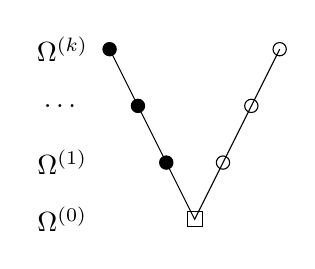
\begin{tikzpicture}[scale=1.2]
% see also fullcycle.tex

  \pgfmathsetmacro\hstep{0.3}
  \pgfmathsetmacro\vstep{0.6}
  \pgfmathsetmacro\ceps{0.08}   % size of square for coarse grid

% grid labels at left
  \node at (-0.5,3*\vstep) {$\Omega^{(k)}$};
  \node at (-0.5,2*\vstep) {\dots};
  \node at (-0.5,\vstep) {$\Omega^{(1)}$};
  \node at (-0.5,0.0) {$\Omega^{(0)}$};

% V-cycle
  \draw[black,thin] (0.0,3*\vstep) -- (\hstep,2*\vstep) --  (2*\hstep,\vstep) -- (3*\hstep,0.0)
                    -- (4*\hstep,\vstep) -- (5*\hstep,2*\vstep) -- (6*\hstep,3*\vstep);
  \filldraw (0.0,3*\vstep) circle (2.0pt);
  \filldraw (\hstep,2*\vstep) circle (2.0pt);
  \filldraw (2*\hstep,\vstep) circle (2.0pt);
  \draw     (3*\hstep-\ceps,-\ceps) rectangle (3*\hstep+\ceps,+\ceps);
  \draw     (4*\hstep,\vstep) circle (2.0pt);
  \draw     (5*\hstep,2*\vstep) circle (2.0pt);
  \draw     (6*\hstep,3*\vstep) circle (2.0pt);

\end{tikzpicture}


\end{minipage}
\end{frame}


\begin{frame}{multigrid uses cheap smoothers}

\begin{itemize}
\item \emph{question}: what does ``improve $\bw$ on the level $l$ grid'' mean?

\emph{answer}: \alert{smoothing}
\item many classical linear iterations are smoothing
	\begin{itemize}
	\item[$\circ$] e.g.~weighted Jacobi and Gauss-Seidel
	\item[$\circ$] fast $O(N)$ operations
	\item[$\circ$] single iteration reduces high-frequency components of the error
	\end{itemize}
\end{itemize}

\begin{center}
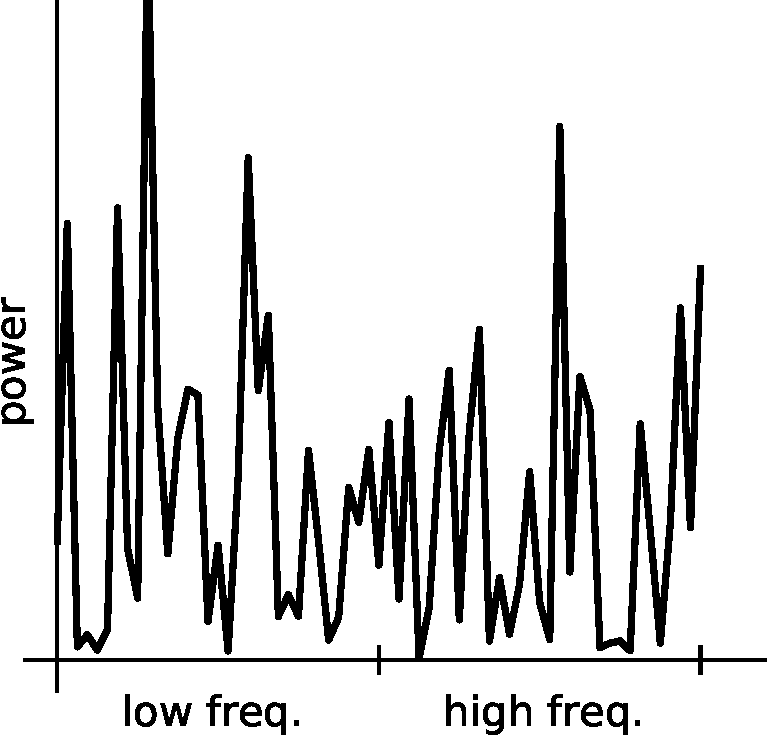
\includegraphics[width=0.25\textwidth]{figs/ps-unsmoothed}

\vspace{-3mm}

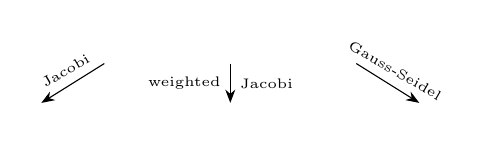
\begin{tikzpicture}[scale=2.0]
  \draw[-Stealth] (-0.8,0.0) -- (-1.2,-0.25) node [midway,rotate=30,above] {\tiny Jacobi};
  \draw[-Stealth] (0.0,0.0) -- (0.0,-0.25) node [midway,left] {\tiny weighted} node [midway,right] {\tiny Jacobi};
  \draw[-Stealth] (0.8,0.0) -- (1.2,-0.25) node [midway,rotate=-30,above] {\tiny Gauss-Seidel};
\end{tikzpicture}

\mbox{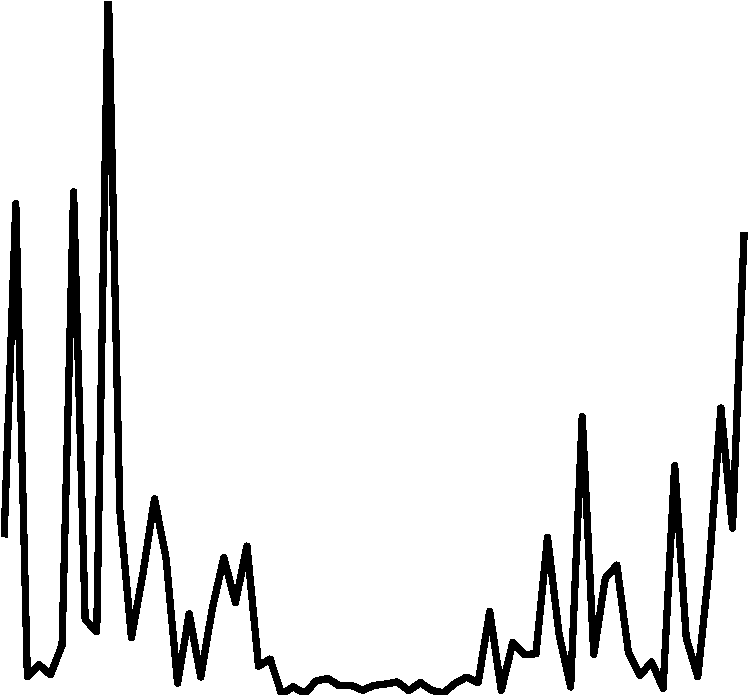
\includegraphics[width=0.2\textwidth]{figs/ps-jacobismoothed} \qquad
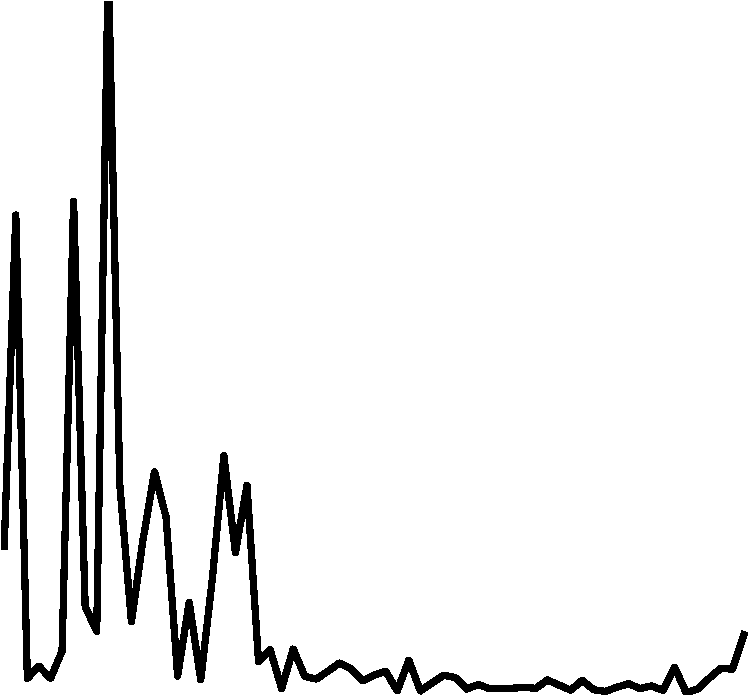
\includegraphics[width=0.2\textwidth]{figs/ps-wjacobismoothed} \qquad
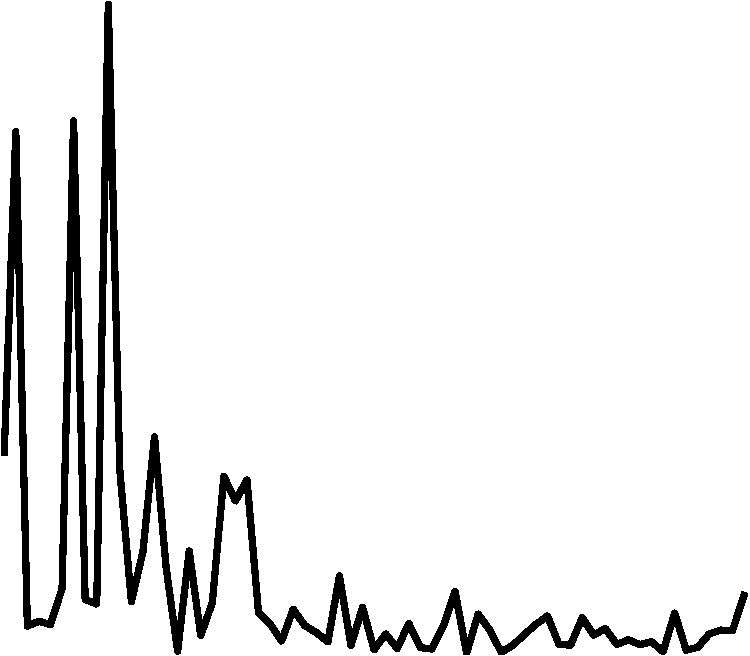
\includegraphics[width=0.2\textwidth]{figs/ps-gssmoothed}}
\end{center}
\end{frame}


\begin{frame}{multigrid: why it is $O(N)$}

\begin{itemize}
\item multigrid is a systematic way of combining two actions
	\begin{itemize}
	\item[$\circ$] \emph{smoothing}: filter out high frequencies of the error on your grid
	\item[$\circ$] \emph{coarsening}: transfer to a smaller-$N$ grid
    	\begin{itemize}
	    \item frequencies that were ``medium-low'' are now ``high''
    	\end{itemize}
	\end{itemize}
\item the work of restricting and interpolating is comparable to the $O(N)$ smoother step
	\begin{itemize}
	\item[$\circ$] total work on $\Omega^{(l)}$ is $C N_l$ for fixed $C$
	\end{itemize}
\item then the total work of a V-cycle is a finite geometric series:

\vspace{-3mm}
\small
\begin{align*}
&(\Omega^{(k)} \text{ work}) + (\Omega^{(k-1)} \text{ work}) + \dots + (\Omega^{(1)} \text{ work}) + (\Omega^{(0)} \text{ work}) \\
&\quad = C N_k + C N_{k-1} + \dots + C N_1 + C_0 \\
&\quad = C N_k + C \frac{N_k}{2^d}  + \dots + C \left(\frac{1}{2^d}\right)^{k-1} N_k + C_0 \\
&\quad \le 2 C N_k + C_0
\end{align*}

    \vspace{-2mm}
	\begin{itemize}
	\item[$\circ$] re the coarsest grid \dots who cares! \dots $C_0$ is independent of $N$
	\end{itemize}

\end{itemize}
\end{frame}

\newcommand{\niceprob}{V-cycle-preconditioned CG iterations on $\Omega=[0,1]^d$ Poisson}
\newcommand{\niceprobtwo}{V-cycle-preconditioned CG iterations on $\Omega=[0,1]^2$ Poisson}

\begin{frame}{multigrid on Poisson}
\begin{itemize}
\item \niceprobtwo
\end{itemize}

\begin{center}
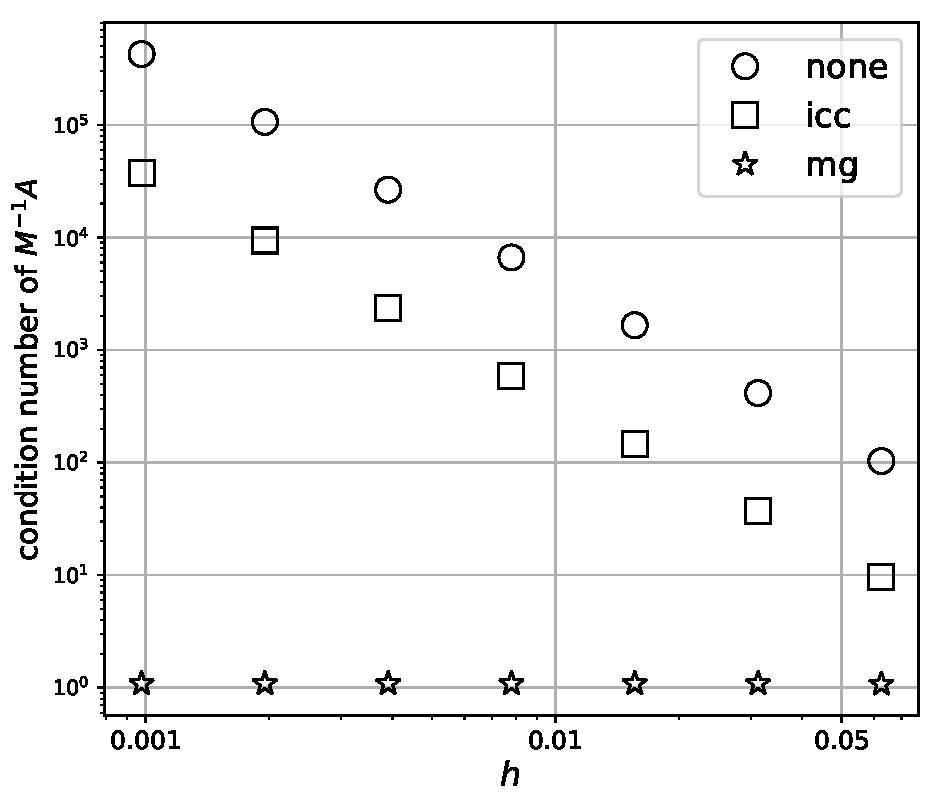
\includegraphics[width=0.6\textwidth]{figs/pccondition}

\small values of $\kappa_2(M^{-1}A)$ for 2D problem
\end{center}
\end{frame}


\begin{frame}{multigrid on Poisson: evidence of optimality}
\begin{itemize}
\item \niceprob
\end{itemize}

\begin{center}
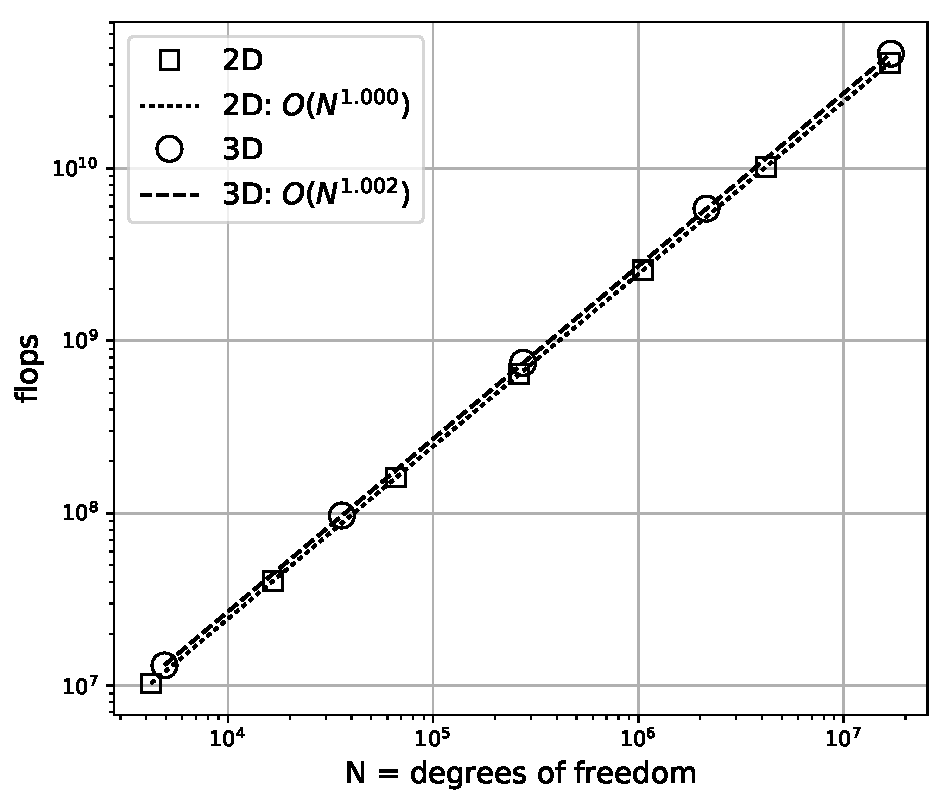
\includegraphics[width=0.6\textwidth]{figs/optimal-flops}

\small direct demonstration of $O(N)$ work
\end{center}
\end{frame}


\begin{frame}{multigrid on Poisson: evidence of optimality}
\begin{itemize}
\item \niceprob
\end{itemize}

\begin{center}
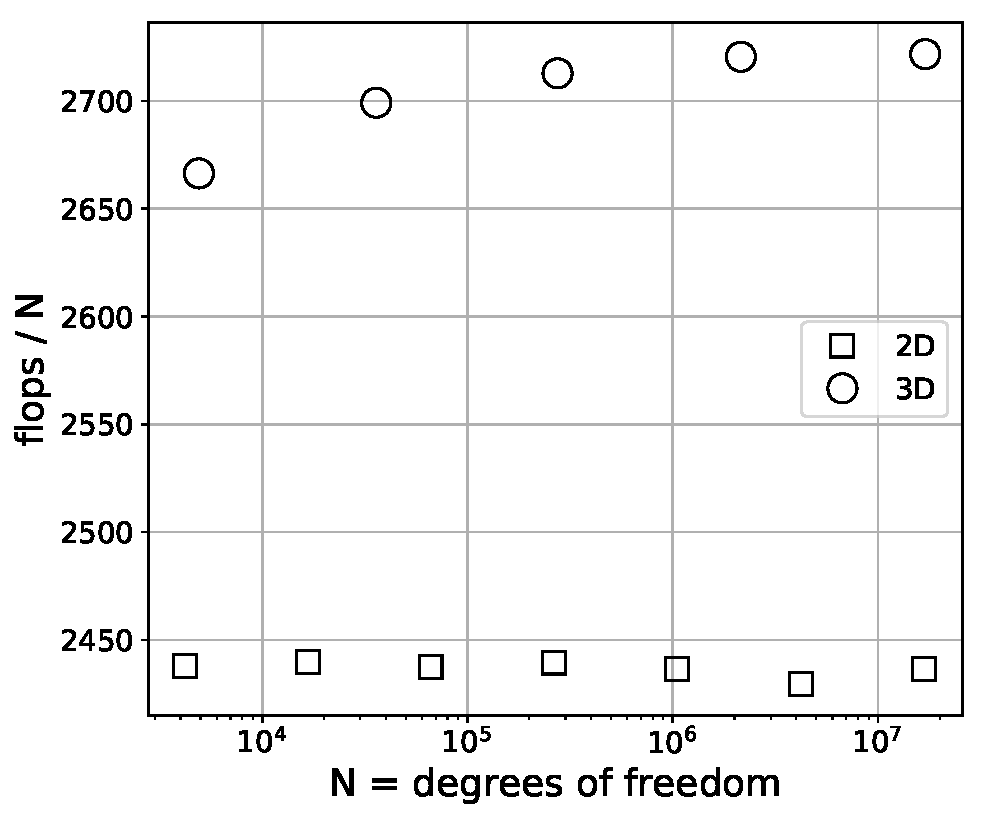
\includegraphics[width=0.6\textwidth]{figs/optimal-flopsperN}

\small i.e.~constant amount of work per degree of freedom
\end{center}
\end{frame}


\begin{frame}{multigrid on Poisson: evidence of optimality}
\begin{itemize}
\item \niceprob
\end{itemize}

\begin{center}
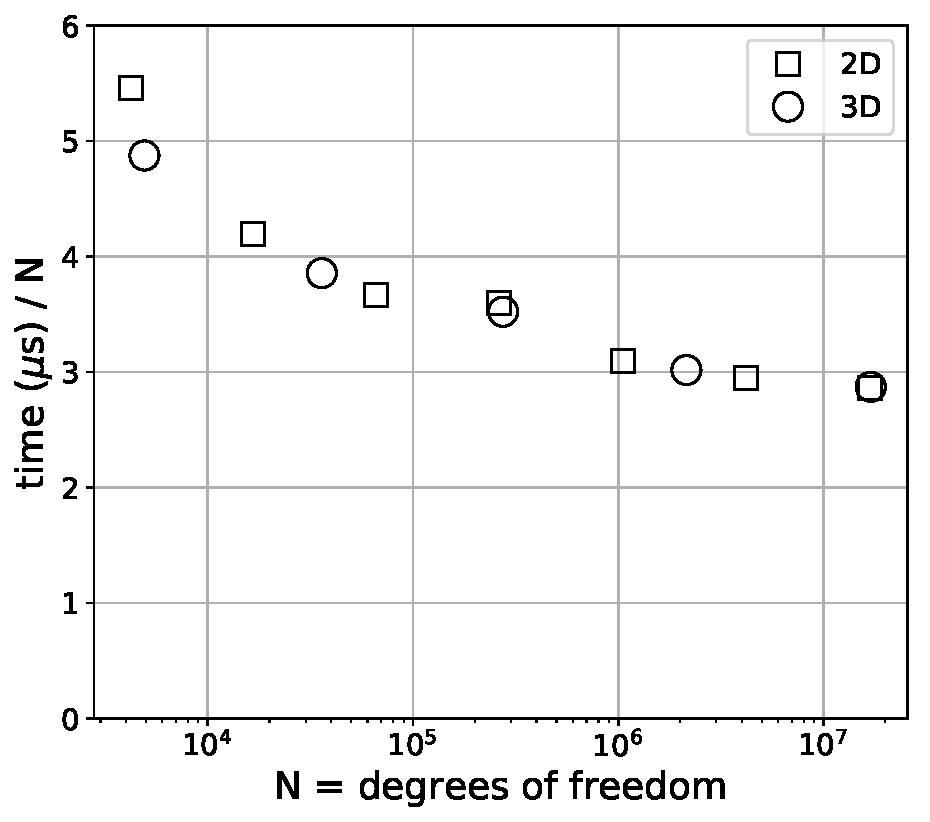
\includegraphics[width=0.6\textwidth]{figs/optimal-timeperN}

\small (almost) constant amount of time per degree of freedom
\end{center}
\end{frame}


\begin{frame}{multigrid on MSE}
\begin{itemize}
\item recall the nonlinear MSE problem on $\Omega=[0,1]^2$:
\small
    $$- \grad\cdot \left(\frac{\grad u}{\sqrt{1 + |\grad u|^2}}\right) = 0  \qquad \text{ with } u\big|_{\partial \Omega} = g.$$
\normalsize
    \vspace{-3mm}
    \begin{itemize}
    \item[$\circ$] solved by Newton iteration
    \item[$\circ$] how to \emph{find a convergent initial iterate} on a fine grid?
    \end{itemize}
\item multigrid solution is by nonlinear ``F-cycle''
    \begin{itemize}
    \item[$\circ$] a.k.a.~nested iteration with V-cycles
    \item[$\circ$] start on coarse grid
    \item[$\circ$] interpolating from coarse grid gives good initial iterate
    \end{itemize}
\end{itemize}

\begin{center}
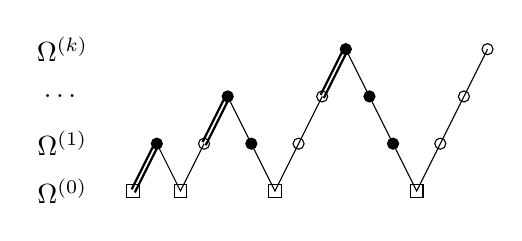
\begin{tikzpicture}[scale=1.0]
% see also vwcycles.tex
  \pgfmathsetmacro\hstep{0.3}
  \pgfmathsetmacro\vstep{0.6}
  \pgfmathsetmacro\ceps{0.08}   % size of square for coarse grid

% grid labels at left
  \node at (-0.0,3*\vstep) {$\Omega^{(k)}$};
  \node at (-0.0,2*\vstep) {$\dots$};
  \node at (-0.0,\vstep) {$\Omega^{(1)}$};
  \node at (-0.0,0.0) {$\Omega^{(0)}$};

  \pgfmathsetmacro\hoff{0*\hstep}
  \draw[shift={(\hoff,0)}]     (3*\hstep-\ceps,-\ceps) rectangle (3*\hstep+\ceps,+\ceps);
  \draw[shift={(\hoff+0.02,-0.02)},black,thick] (3*\hstep,0.0) -- (4*\hstep,\vstep);
  \draw[shift={(\hoff-0.02,0.02)},black,thick] (3*\hstep,0.0) -- (4*\hstep,\vstep);

% V-cycle to level 1
  \pgfmathsetmacro\hoff{4*\hstep}
  \draw[shift={(\hoff,0)},black,thin] (0.0,\vstep) -- (\hstep,0.0) -- (2*\hstep,\vstep);
  \draw[shift={(\hoff+0.02,-0.02)},black,thick] (2*\hstep,\vstep) -- (3*\hstep,2*\vstep);
  \draw[shift={(\hoff-0.02,+0.02)},black,thick] (2*\hstep,\vstep) -- (3*\hstep,2*\vstep);
  \filldraw[shift={(\hoff,0)}] (0.0,\vstep) circle (2.0pt);
  \draw[shift={(\hoff,0)}]     (\hstep-\ceps,-\ceps) rectangle (\hstep+\ceps,+\ceps);
  \draw[shift={(\hoff,0)}]     (2*\hstep,\vstep) circle (2.0pt);

% V-cycle to level 2
  \pgfmathsetmacro\hoff{7*\hstep}
  \draw[shift={(\hoff,0)},black,thin] (0.0,2*\vstep) --  (\hstep,\vstep) -- (2*\hstep,0.0) -- (3*\hstep,\vstep) -- (4*\hstep,2*\vstep);
  \draw[shift={(\hoff+0.02,-0.02)},black,thick] (4*\hstep,2*\vstep) -- (5*\hstep,3*\vstep);
  \draw[shift={(\hoff-0.02,+0.02)},black,thick] (4*\hstep,2*\vstep) -- (5*\hstep,3*\vstep);
  \filldraw[shift={(\hoff,0)}] (0.0,2*\vstep) circle (2.0pt);
  \filldraw[shift={(\hoff,0)}] (\hstep,\vstep) circle (2.0pt);
  \draw[shift={(\hoff,0)}]     (2*\hstep-\ceps,-\ceps) rectangle (2*\hstep+\ceps,+\ceps);
  \draw[shift={(\hoff,0)}]     (3*\hstep,\vstep) circle (2.0pt);
  \draw[shift={(\hoff,0)}]     (4*\hstep,2*\vstep) circle (2.0pt);

% V-cycle to finest (level 3)
  \pgfmathsetmacro\hoff{12*\hstep}
  \draw[shift={(\hoff,0)},black,thin] (0.0,3*\vstep) -- (\hstep,2*\vstep) --  (2*\hstep,\vstep) -- (3*\hstep,0.0)
                    -- (4*\hstep,\vstep) -- (5*\hstep,2*\vstep) -- (6*\hstep,3*\vstep);
  \filldraw[shift={(\hoff,0)}] (0.0,3*\vstep) circle (2.0pt);
  \filldraw[shift={(\hoff,0)}] (\hstep,2*\vstep) circle (2.0pt);
  \filldraw[shift={(\hoff,0)}] (2*\hstep,\vstep) circle (2.0pt);
  \draw[shift={(\hoff,0)}]     (3*\hstep-\ceps,-\ceps) rectangle (3*\hstep+\ceps,+\ceps);
  \draw[shift={(\hoff,0)}]     (4*\hstep,\vstep) circle (2.0pt);
  \draw[shift={(\hoff,0)}]     (5*\hstep,2*\vstep) circle (2.0pt);
  \draw[shift={(\hoff,0)}]     (6*\hstep,3*\vstep) circle (2.0pt);


\end{tikzpicture}
\end{center}
\end{frame}


\begin{frame}{multigrid on MSE: evidence of optimality}

\begin{center}
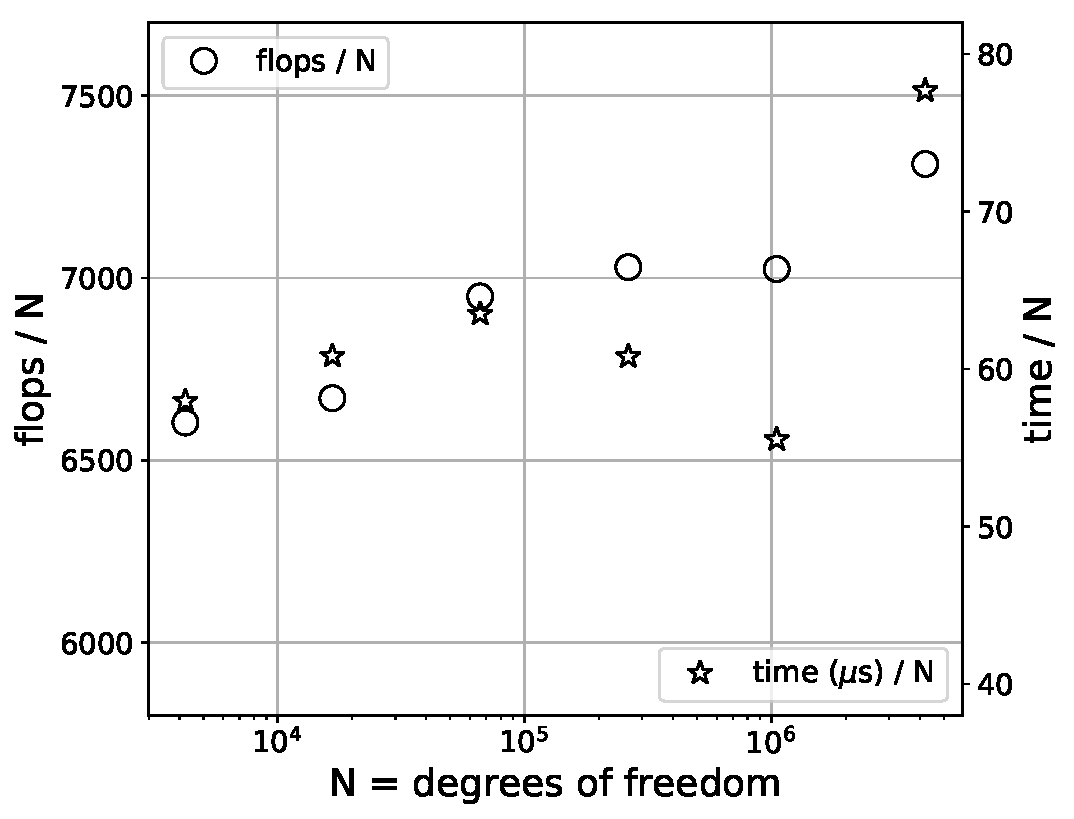
\includegraphics[width=0.6\textwidth]{figs/minoptimal}
\end{center}
\begin{itemize}
\item on finest $2049\times 2049$ grid with $N=4\times 10^6$:
    $$\text{total flops} = N \, \left(\frac{\text{flops}}{N}\right) = (4\times 10^6) (7 \times 10^3) \approx 3 \times 10^{10}$$
    \vspace{-3mm}
    \begin{itemize}
    \item[$\circ$] runtime about 5 minutes total
    \end{itemize}
\end{itemize}
\end{frame}


\begin{frame}{algebraic multigrid}
\begin{itemize}
\item FIXME   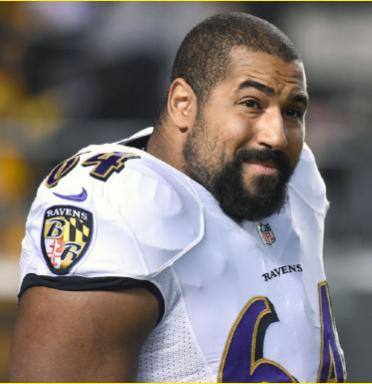
\includegraphics[width=0.2\textwidth]{figs/urschel}
\end{itemize}
\end{frame}


\begin{frame}{algebraic multigrid}
\begin{itemize}
\item FIXME   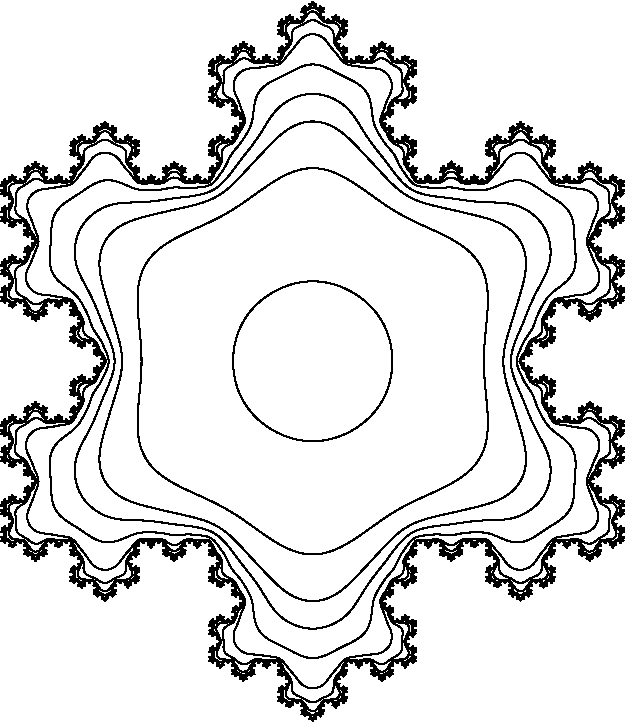
\includegraphics[width=0.3\textwidth]{figs/snowflake}
\end{itemize}

\begin{center}
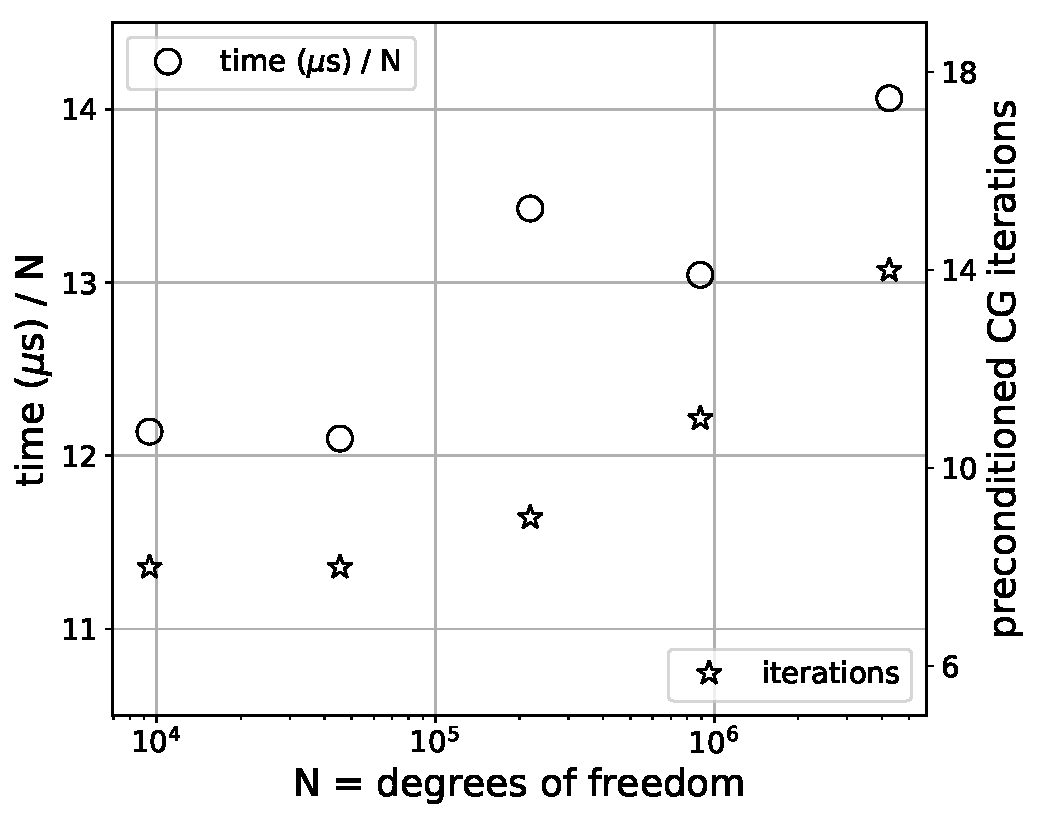
\includegraphics[width=0.5\textwidth]{figs/gamgopt}
\end{center}
\end{frame}


\section{nonlinear problems and unstructured grids}

\begin{frame}{wider applicability of multigrid}

\begin{columns}
\begin{column}{0.8\textwidth}
\begin{itemize}
\item multigrid was invented for Poisson and linear elliptic equations by Federenko (1962, 1964)
\item apparently, by 1975 optimism about multigrid was limited to one person: Achi Brandt
\item faith in its wider applicability has been growing every since
\end{itemize}
\end{column}

\begin{column}{0.15\textwidth}


\includegraphics[width=\textwidth]{figs/starwars-achi-mashup.jpg}
\end{column}
\end{columns}
\end{frame}

\begin{frame}{FIXME}
\begin{itemize}
\item FIXME
\end{itemize}
\end{frame}



\section{barriers}


\begin{frame}{low regularity of solution}
\begin{itemize}
\item again assume solution of (nonlinear) BVP on $\Omega \subset \RR^d$
\item $W(h)$ Newton iterations
\item $K(h)$ preconditioned Krylov steps per Newton
\item FIXME  in some case number of Newton steps (or Krylov steps) now grows as $h\to 0$
\item can demo w MSE  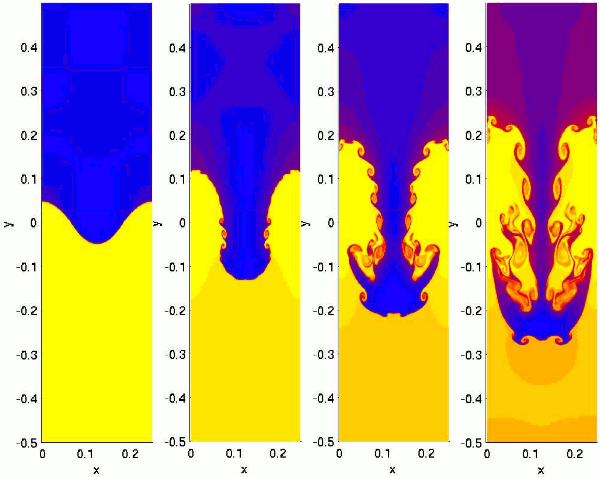
\includegraphics[width=0.4\textwidth]{figs/rayleigh-taylor-instability}
\end{itemize}
\end{frame}


\begin{frame}{constrained problems}
\begin{itemize}
\item FIXME  number of Newton steps proportional to $D/h$ where $D$ is distance-to-move free boundary
\item Max working on it
\end{itemize}
\end{frame}


\section{extensions}


\begin{frame}{when is optimality the right concept?}
\begin{itemize}
\item so far the
    \begin{itemize}
    \item[$\circ$] problems are elliptic PDE BVPs
    \item[$\circ$] algorithms are serial
    \end{itemize}
\item is the question of optimality useful more broadly?
\end{itemize}
\end{frame}


\begin{frame}{hyperbolic PDE IBVPs}
\begin{itemize}
\item FIXME
\end{itemize}
\end{frame}


\begin{frame}{initial/boundary value problems}

\begin{itemize}
\item consider a problem posed on $\Omega \times [0,T]$ where $\Omega \subset \RR^d$
    \begin{itemize}
    \item[$\circ$] hyperbolic example: nonlinear wave equation (system)
      $$FIXME$$
    \item[$\circ$] general example: nonlinear convection/diffusion/reaction equation
      $$u_t = \Div(a(u) \grad u) - b(u)\cdot \grad u + f(u)$$
    \item[$\circ$] evolution problem with states in some $\infty$-dimensional (Sobolev) space
    \end{itemize}
\item what should ``optimal'' mean?
\end{itemize}
\end{frame}


\begin{frame}{numerical parameters for IBVPs}

\begin{itemize}
\item assume structured spatial grid: $h=\Delta x = \Delta y=\Delta z$
    \begin{itemize}
    \item[$\circ$] $N=$ (spatial degrees of freedom) $=O(h^{-d})$
    \end{itemize}
\item time step is limited in some way \dots almost always:
    $$\Delta t \le O(h^q)$$
    \vspace{-5mm}
    \begin{itemize}
    \item[$\circ$] stability: $q=2$ for explicit schemes on diffusions
	    \begin{itemize}
	    \item explicit schemes clearly not optimal
	    \end{itemize}
    \item[$\circ$] accuracy: usually $q=1$
	    \begin{itemize}
	    \item e.g.~for $O(h^2+\Delta t^2)$ methods
	    \end{itemize}
    \item[$\circ$] movie: generate $M$ frames, so $\Delta t = T/M$
    \item[$\circ$] ``total number of degrees of freedom'' $=M N$?
    \end{itemize}
\item (implicit) solution for one time step using NK:
    \begin{itemize}
    \item[$\circ$] $W(h)$ Newton iterations
    \item[$\circ$] $K(h)$ preconditioned Krylov steps per Newton
    \item[$\circ$] $W(h)=K(h)=1$ for explicit methods
    \end{itemize}
\end{itemize}
\end{frame}


\begin{frame}{optimality(?) for IBVPs}

\begin{itemize}
\item FIXME for hyperbolic where $\Delta t \sim \Delta x$, explicit schemes already optimal
\item yields: a ``performance model'' for solving IBVPs on $\Omega \times [0,T]$
\item cost of computation:
\footnotesize
\begin{align*}
C &= (\text{number of steps}) \cdot (\text{iterations per step}) \cdot (\text{cost of 1 spatial residual}) \\
  &= O(h^{-q}) \cdot W(h) \, K(h) \cdot O(h^{-d})
\end{align*}
\normalsize
\item we define solver to be \emph{optimal} if work is $O(MN)$?
    \begin{itemize}
    \item[$\circ$] optimal movie-limited (implicit) steps:
        $$C = M \cdot W \cdot O(1) \cdot O(h^{-d}) = O(MN)$$
    \item[$\circ$] optimal accuracy-limited (implicit) steps:
        $$C = O(h^{-1}) \cdot W \cdot O(1) \cdot O(h^{-d}) = O(N^{1+1/d})$$
    \item[$\circ$] explicit:
        $$C = O(h^{-2}) \cdot 1 \cdot 1 \cdot O(h^{-d}) = O(N^{1+2/d}) \hfill \alert{\leftarrow \text{ beat this!?}}$$
    \end{itemize}
\end{itemize}
\end{frame}


\begin{frame}{contrast: spectral methods}
\begin{itemize}
\item FIXME
\item spectral methods show that pursuit of optimality is \emph{not} the only good goal
\end{itemize}
\end{frame}


\begin{frame}{goal of parallel scaling}
\begin{itemize}
\item FIXME not exactly a ``barrier'' but a conflict
\end{itemize}

\begin{center}
\only<1>{\hspace{0mm}}
\includegraphics<1>[width=0.6\textwidth]{figs/NPplane}
\includegraphics<2>[width=0.6\textwidth]{figs/NPplanestatic}
\includegraphics<3>[width=0.6\textwidth]{figs/NPplaneweakstrong}
\end{center}
\end{frame}


\begin{frame}{conclusion}
\begin{itemize}
\item in approximately solving your PDE-type problem on a modern computer, as you head toward $N=\infty$ unknowns,

\bigskip
\begin{quote}
\alert{you should be solving the $N$ equations in $O(N)$ work}
\end{quote}

\bigskip
\item this is a good \emph{goal} for PDE BVPs
\item \dots but you must exploit
    \begin{itemize}
    \item[$\circ$] the locality (sparsity) of the problem, and
    \item[$\circ$] correlation (smoothness) of the solution
    \end{itemize}
\item multigrid is the only hope!?

\bigskip
\item for general dense systems $A\bu=\bb$ the goal is $O(N^2)$?
    \begin{itemize}
    \item[$\circ$] how to get there is an open problem
    \end{itemize}
\end{itemize}
\end{frame}


\end{document}
